\subsection{问题一：数据质量评价与领域配比建模}
\begingroup
\captionsetup[figure]{font={bundledsong,minusfour,bf}}
\captionsetup[table]{font={bundledsong,minusfour,bf}}
\widowpenalty=10000
\clubpenalty=10000
\emergencystretch=1em

\subsubsection{具体分析}

本问首先要把 22 个不同形式的质量信号整理成统一评分，再判断这些指标是否会对同一文本给出相反评价。我们采用熵权法计算样本、语料和领域评分，用成对标准化得分差及 Kendall 协同系数分析评价分歧。在此基础上，另用岭正则线性混合回归研究 17 个训练领域的占比与 13 个验证领域损失的关系\cite{liu2024regmix}，为后续选择语料配方提供依据。

图\ref{fig:q1_workflow}将处理过程分为质量评价和配比分析两部分。前者读取 A1--A3，依次处理缺失值、将列表指标转为标量、统一方向并归一化，随后计算评分与冲突情况。后者按索引连接训练配方和验证损失，拟合岭回归，利用 1M、60M、1B 检验集及 10B、70B 外推表比较结果，再求出有界推荐配比。两部分通过领域映射表对应。

\begin{figure}[htbp]
  \centering
  % 只展示已有实现：冲突诊断不等同于已完成样本消解或降权。
\begingroup
\definecolor{qflowblue}{HTML}{315A79}
\definecolor{qflowlight}{HTML}{EDF3F7}
\definecolor{qflowgray}{HTML}{536572}
\begin{tikzpicture}[
  font=\song\fontsize{10}{13}\selectfont,
  qbox/.style={draw=qflowblue!55, line width=0.55pt, rounded corners=2pt,
    fill=qflowlight, align=center, inner sep=7pt, minimum height=1.15cm},
  qwide/.style={qbox, text width=6.0cm},
  qhalf/.style={qbox, text width=2.55cm, minimum height=1.7cm},
  qlink/.style={-{Stealth[length=2mm]}, draw=qflowblue, line width=0.7pt},
  qhead/.style={text=qflowblue, font=\song\bfseries\fontsize{11}{14}\selectfont}
]
\node[qhead] at (-3.9,0.9) {质量评价流程};
\node[qhead] at (3.9,0.9) {配比建模流程};
\node[qwide, fill=qflowblue, text=white] (quality) at (-3.9,0)
  {A1--A3 质量信号\\22 个指标与文本领域信息};
\node[qwide, fill=qflowblue, text=white] (mixture) at (3.9,0)
  {A4--A5 训练配方与验证损失\\17 个训练领域、13 个验证领域};

\node[qwide] (prepare) at (-3.9,-1.95)
  {缺失值处理与列表标量化\\统一指标方向并进行归一化};
\node[qwide] (match) at (3.9,-1.95)
  {按 index 匹配配方与损失\\构造配比矩阵 $\bm P$ 与损失矩阵 $\bm L$};

\node[qhalf] (score) at (-5.62,-4.15)
  {熵权综合评价\\样本、语料和领域\\质量评分};
\node[qhalf] (conflict) at (-2.18,-4.15)
  {指标冲突诊断\\成对标准化分数差\\Kendall 一致性};
\node[qwide] (ridge) at (3.9,-4.15)
  {岭正则线性混合回归\\估计回归系数并预测验证损失};

\node[qwide, fill=white] (mapping) at (-3.9,-6.55)
  {A16 领域映射\\构造混合质量指数 $\bar Q(\bm p)$};
\node[qwide] (validation) at (3.9,-6.55)
  {模型检验与跨尺度分析\\1M 检验、60M/1B 相关性\\10B/70B 外推表};
\node[qwide, fill=white] (recommend) at (3.9,-8.75)
  {有界配比推荐\\固定未测量域、设置配比上限};

\draw[qlink] (quality) -- (prepare);
\draw[qflowblue, line width=0.7pt] (prepare.south) -- (-3.9,-2.95);
\draw[qlink] (-3.9,-2.95) -| (score.north);
\draw[qlink] (-3.9,-2.95) -| (conflict.north);
\draw[qlink] (score.south) -- (-5.62,-5.7) -| (mapping.north);

\draw[qlink] (mixture) -- (match);
\draw[qlink] (match) -- (ridge);
\draw[qlink] (ridge) -- (validation);
\draw[qlink] (validation) -- (recommend);
\draw[qlink, dashed] (mapping.east) -- (0,-6.55) -- (0,-4.15) -- (ridge.west);
\node[fill=white, text=qflowgray, align=center, inner sep=2pt,
  font=\song\fontsize{8.5}{11}\selectfont] at (0,-5.35) {质量项\\增量检验};

\node[align=left, text=qflowgray, text width=6.0cm,
  font=\song\fontsize{9}{12}\selectfont] at (-3.9,-8.6)
  {实线表示主要处理流程；虚线表示混合质量指数的追加检验。};
\end{tikzpicture}
\endgroup

  \caption{问题一的质量评价与领域配比建模流程}
  \label{fig:q1_workflow}
\end{figure}

\subsubsection{模型准备}

\Needspace{4\baselineskip}
\textbf{1. 数据来源与预处理}\par\nopagebreak[4]

配比分析使用 A4 和 A5。A4 的每一行表示一组 The Pile 训练配方，包含 17 个非负占比，合计为 1\cite{gao2020pile}；A5 记录该配方在 13 个验证领域的交叉熵损失，按 index 与 A4 连接。训练领域中的 nih\_\allowbreak{}exporter、enron\_\allowbreak{}emails、europarl 和 philpapers 没有各自的验证损失列。我们仍保留它们的占比，用“间接影响域”表示这四类领域，解释系数时不将其当作独立验证目标。

A1--A3 提供 SlimPajama 语料的 22 个质量指标\cite{slimpajama2025}。为使各指标能够共同参与评分，需要统一其方向。设第 $j$ 个指标的原始值为 $x_j$，正向指标作极差归一化，负向指标反向缩放；对于过长或过短均不合适的长度型指标，使用其与稳健中心的接近程度表示质量：
\begin{equation}
    x'_j = \begin{cases}
        \dfrac{x_j-\min x_j}{\max x_j-\min x_j}, & \text{正向指标}\\[6pt]
        \dfrac{\max x_j-x_j}{\max x_j-\min x_j}, & \text{负向指标}\\[6pt]
        \exp\!\left(-\dfrac{|\ln(1+x_j)-m_j|}{2.5\,\text{MAD}_j}\right), & \text{长度型指标}
    \end{cases}
\end{equation}
式中，$m_j$ 为取对数后的中位数，$\text{MAD}_j$ 为相应的中位绝对偏差。变换后的 $x'_j$ 均落在 $[0,1]$，并统一为高分表示较高质量。8 个列表型指标先按有序类别 logits 计算 softmax 概率，再求归一化期望级别，将多维信息转成一个数值后参与归一化。各字段的含义、方向和最终权重见表\ref{tab:p1_dir}。

\begingroup
\setlength{\tabcolsep}{3pt}
\begin{longtable}{@{}>{\raggedright\arraybackslash}p{0.33\textwidth}>{\centering\arraybackslash}p{0.10\textwidth}>{\raggedright\arraybackslash}p{0.31\textwidth}>{\centering\arraybackslash}p{0.08\textwidth}>{\centering\arraybackslash}p{0.10\textwidth}@{}}
  \caption{质量指标的含义、评价方向及熵权}
  \label{tab:p1_dir} \\
  \toprule
  指标字段 & 类型 & 指标含义与判向依据 & 方向 & 熵权 $w_j$ \\
  \midrule
  \endfirsthead
  \caption{质量指标的含义、评价方向及熵权（续）} \\
  \toprule
  指标字段 & 类型 & 指标含义与判向依据 & 方向 & 熵权 $w_j$ \\
  \midrule
  \endhead
  \bottomrule
  \endfoot
  fineweb\_\allowbreak{}edu & 列表(1) & 文本用于教育的价值 & 正向 & 0.0437 \\
  fluency\_\allowbreak{}en & 列表(2) & 英语流畅度（第 1 类=流畅，已核验） & 正向 & 0.0682 \\
  modernbert\_\allowbreak{}cleanliness & 列表(6) & 文本内容的洁净程度 & 正向 & 0.1434 \\
  modernbert\_\allowbreak{}readability & 列表(6) & 文本的易读程度 & 正向 & 0.0567 \\
  modernbert\_\allowbreak{}reasoning & 列表(6) & 内容体现的推理程度 & 正向 & \textbf{0.1517} \\
  modernbert\_\allowbreak{}professionalism & 列表(6) & 内容的专业程度 & 正向 & 0.0396 \\
  dsir\_\allowbreak{}books & 标量 & 相对于书籍领域的重要性权重 & 正向 & 0.0081 \\
  dsir\_\allowbreak{}wiki & 标量 & 相对于维基领域的重要性权重 & 正向 & 0.0081 \\
  dsir\_\allowbreak{}math & 标量 & 相对于数学领域的重要性权重 & 正向 & 0.0086 \\
  qurater & 列表(4) & 教育质量评级（4 项取均值） & 正向 & 0.0492 \\
  ad\_\allowbreak{}en & 列表(2) & 广告含量（\textbf{第 1 类=“无广告”，正向}；依据：原文抽查） & 正向 & 0.0072 \\
  rps\_\allowbreak{}doc\_\allowbreak{}word\_\allowbreak{}count & 标量 & 文档包含的词总数 & 长度型 & 0.0516 \\
  rps\_\allowbreak{}doc\_\allowbreak{}num\_\allowbreak{}sentences & 标量 & 文档包含的句子总数 & 长度型 & 0.0523 \\
  rps\_\allowbreak{}doc\_\allowbreak{}unigram\_\allowbreak{}entropy & 标量 & 用一元词熵衡量词汇多样性 & 正向 & 0.0347 \\
  rps\_\allowbreak{}doc\_\allowbreak{}frac\_\allowbreak{}unique\_\allowbreak{}words & 标量 & 不同词项所占比例 & 正向 & 0.0538 \\
  rps\_\allowbreak{}doc\_\allowbreak{}frac\_\allowbreak{}no\_\allowbreak{}alph\_\allowbreak{}words & 标量 & 非字母字符所占比例 & 负向 & 0.0287 \\
  rps\_\allowbreak{}doc\_\allowbreak{}frac\_\allowbreak{}chars\_\allowbreak{}top\_\allowbreak{}2gram & 标量 & 字符 2-gram 的重复程度 & 负向 & 0.0130 \\
  rps\_\allowbreak{}doc\_\allowbreak{}frac\_\allowbreak{}chars\_\allowbreak{}top\_\allowbreak{}3gram & 标量 & 字符 3-gram 的重复程度 & 负向 & 0.0119 \\
  rps\_\allowbreak{}lines\_\allowbreak{}uppercase\_\allowbreak{}letter\_\allowbreak{}fraction & 标量 & 大写字母行所占比例 & 负向 & 0.0316 \\
  rps\_\allowbreak{}lines\_\allowbreak{}ending\_\allowbreak{}with\_\allowbreak{}terminal\_\allowbreak{}punctution\_\allowbreak{}mark & 标量 & 以终止标点结束的行所占比例 & 正向 & 0.0880 \\
  rps\_\allowbreak{}lines\_\allowbreak{}numerical\_\allowbreak{}chars\_\allowbreak{}fraction & 标量 & 含有数字的行所占比例 & 负向 & 0.0125 \\
  rps\_\allowbreak{}doc\_\allowbreak{}mean\_\allowbreak{}word\_\allowbreak{}length & 标量 & 词项长度的平均值 & 长度型 & 0.0373 \\
\end{longtable}
\endgroup

在统一指标方向后，以加权和计算样本质量 $Q_i$，再对同一领域内的样本取均值，得到领域质量 $Q_d$：
\begin{equation}
    Q_i = \sum_{j=1}^{22} w_j\, x'_{ij},\qquad Q_d=\frac{1}{n_d}\sum_{i\in\mathcal D_d}Q_i,\qquad \sum_j w_j=1
\end{equation}
表\ref{tab:p1_dir}中，modernbert\_\allowbreak{}reasoning 与 modernbert\_\allowbreak{}cleanliness 的熵权分别为 $0.152$、$0.143$，对综合分数的作用较大。这里的 $w_j$ 由指标分布确定，反映的是熵权法所衡量的信息差异。由于极端左偏分布也可能获得较大权重，评分结果还需与其他赋权方式比较，第\ref{sec:check}节给出相应检验。

计算前逐字段检查质量信号，缺失统计见表\ref{tab:p1_missing}。对缺失位置填入该指标的中位数，使缺失本身不被记为高分或低分。

\begingroup
\setlength{\tabcolsep}{3pt}
\begin{longtable}{@{}>{\raggedright\arraybackslash}p{0.44\textwidth}>{\centering\arraybackslash}p{0.16\textwidth}>{\raggedright\arraybackslash}p{0.36\textwidth}@{}}
  \caption{A1--A3 中 272{,}505 条记录的质量字段缺失统计}
  \label{tab:p1_missing} \\
  \toprule
  缺失字段 & 涉及记录数 & 缺失情况 \\
  \midrule
  \endfirsthead
  \caption{质量字段缺失统计（续）} \\
  \toprule
  缺失字段 & 涉及记录数 & 缺失情况 \\
  \midrule
  \endhead
  \bottomrule
  \endfoot
  modernbert\_\allowbreak{}reasoning & 13 & 该记录中此字段的 6 个分量均为 NaN \\
  modernbert\_\allowbreak{}professionalism & 6 & 该记录中此字段的 6 个分量均为 NaN \\
  其余 20 个指标 & 0 & 未发现缺失值 \\
\end{longtable}
\endgroup

\Needspace{4\baselineskip}
\textbf{2. 方法选择及其依据}\par\nopagebreak[4]

综合评分分别尝试熵权法、等权平均和 PCA 第一主成分，表\ref{tab:algo1}列出比较结果。指标冲突从两个角度考察：成对标准化得分差用于定位单条文本的评价分歧，Kendall 协同系数用于概括整体排序。配比回归的备选方法包括普通最小二乘、岭回归与随机森林。

\begingroup
\setlength{\tabcolsep}{3pt}
\begin{longtable}{@{}>{\centering\arraybackslash}p{0.20\textwidth}>{\centering\arraybackslash}p{0.16\textwidth}>{\centering\arraybackslash}p{0.20\textwidth}>{\raggedright\arraybackslash}p{0.36\textwidth}@{}}
  \caption{不同赋权方式下的样本得分及领域排序比较}
  \label{tab:algo1} \\
  \toprule
  赋权方法 & 样本平均得分 & 与熵权得分的相关系数 & 领域排序相关性\newline Spearman 系数，参照熵权法 \\
  \midrule
  \endfirsthead
  \caption{不同赋权方式下的样本得分及领域排序比较（续）} \\
  \toprule
  赋权方法 & 样本平均得分 & 与熵权得分的相关系数 & 领域排序相关性\newline Spearman 系数，参照熵权法 \\
  \midrule
  \endhead
  \bottomrule
  \endfoot
  熵权法 & 0.495 & 1.000 & 1.000 \\
  等权平均 & 0.639 & 0.854 & 0.679 \\
  PCA 第一主成分 & 0.520 & 0.881 & 0.679 \\
\end{longtable}
\endgroup

由表\ref{tab:algo1}可见，等权与熵权得分的样本相关系数为 $0.854$，领域排序的 Spearman 系数为 $0.679$。两种方法得到的总体趋势接近，但个别领域的次序会变化。本文选用熵权法，让指标在样本中的信息差异决定权重，并在后文继续检查赋权变化的影响。PCA 能够压缩维度、减少相关信息，但第一主成分较难直接解释为文本质量，因此不作为最终评分方案。

选择岭回归还与配方的约束有关。17 个占比之和恒为 1，一个分量增加必然伴随其他分量减少，直接回归容易出现系数不稳定。加入 $L_2$ 正则后，可以在保留线性解释的同时稳定估计。冲突分析则分别保留样本分歧和整体一致性两个结果，避免用单一统计量代替全部判断。

\subsubsection{模型建立}

\Needspace{4\baselineskip}
\textbf{1. 综合质量评分}\par\nopagebreak[4]

设共有 $m$ 条文本，将其 22 个指标按上述规则处理后组成矩阵 $\bm X=(x'_{ij})$。先根据每列的样本分布求信息熵 $e_j$，再把各列的信息差异换算成权重 $w_j$：
\begin{equation}
    e_j = -\frac{1}{\ln m}\sum_{i=1}^{m} f_{ij}\ln f_{ij},\qquad f_{ij}=\frac{x'_{ij}+\varepsilon}{\sum_i (x'_{ij}+\varepsilon)},\qquad
    w_j = \frac{1-e_j}{\sum_{j=1}^{22}(1-e_j)}
\end{equation}
文本评分之外，损失数据还提供了另一种比较依据：在平均配方下，某验证域的损失越低，说明该域在当前训练条件下越容易拟合。为便于与附件 B 联系，将这一难度差异转换为质量代理值：
\begin{equation}
    Q_d^{(\text{loss})}=1-\frac{\bar L_d-\min_d \bar L_d}{\max_d \bar L_d-\min_d \bar L_d}
\end{equation}
这里用 $\bar L_d$ 表示领域 $d$ 的平均交叉熵损失。该代理值只适用于有损失记录的 13 个领域，而 A1--A3 的文本质量分为 7 个领域。我们依据 A16 连接两套分类，并在求解结果中比较两种评分的排序。

\Needspace{4\baselineskip}
\textbf{2. 质量冲突的定义与处理}\par\nopagebreak[4]

同一文本在两个指标上得分相差较大时，综合评价可能受到分歧影响。为识别这种情况，先对已统一方向的指标作标准化，再计算样本 $i$ 在指标 $j$、$k$ 之间的距离：
\begin{equation}
    \delta_i(j,k) = \left| z_{ij} - z_{ik} \right|,\qquad z_{ij}=\frac{x'_{ij}-\mu_j}{\sigma_j},\qquad
    \mathbf 1\{\delta_i(j,k)>\tau\}
\end{equation}
取阈值 $\tau=1.5$；全样本冲突率为
\begin{equation}
    \rho_c = \frac{1}{m\binom{22}{2}}\sum_{i=1}^{m}\sum_{j<k}\mathbf 1\{\delta_i(j,k)>\tau\}
\end{equation}
仅有冲突率还难以判断分歧程度，因此设置独立标准正态指标的参照 $\rho_0=2\Phi(-\tau/\sqrt2)$。比值 $\rho_c/\rho_0<1$ 表示观察到的冲突少于这一基准，可与整体排序结果共同解释。排序一致性采用 Kendall 协同系数，将 22 个指标看作评价者、$m$ 条文本看作评价对象：
\begin{equation}
    W = \frac{12\sum_i (R_i-\bar R)^2}{22^2\,(m^3-m)},\qquad R_i=\sum_{j=1}^{22} r_{ij},\qquad
    \chi^2 = 22(m-1)W
\end{equation}
$r_{ij}$ 表示样本 $i$ 在指标 $j$ 下的排序。对已标记的冲突样本，本文以加权分数 $Q_i$ 高于还是低于所在领域中位数作综合判断，将其称为“多数指标方向裁决”。同时保留冲突标记，使后续使用者能够识别这类样本，并按需要剔除或降低权重。

\Needspace{4\baselineskip}
\textbf{3. 领域配比的线性混合回归}\par\nopagebreak[4]

把各组训练配方排列为 $\bm P\in[0,1]^{n\times17}$，每行分量相加为 1；相应验证损失组成 $\bm L\in\mathbb R^{n\times13}$。我们分别对每个验证领域建立损失关于训练占比的线性关系：
\begin{equation}
    L_{d}(\bm p) = \sum_{k=1}^{17} a_{dk}\, p_k + b_d,\qquad d=1,\dots,13
\end{equation}
其矩阵形式为
\begin{equation}
    \hat{\bm L} = \bm P \bm A + \bm 1 \bm b^{\top}
\end{equation}
由于 $\bm P$ 的行和固定为 1，截距与配比系数不能仅凭普通回归唯一分开。为稳定求解，对 $\bm A\in\mathbb R^{17\times 13}$ 加入岭惩罚，并共同估计截距 $\bm b$：
\begin{equation}
    \min_{\bm A,\bm b}\ \left\|\bm L-\bm P\bm A-\bm 1\bm b^{\top}\right\|_F^2 + \lambda\left\|\bm A\right\|_F^2
\end{equation}
相应的系数估计为
\begin{equation}
    \begin{bmatrix}\bm A\\ \bm b^{\top}\end{bmatrix}
    = \left(\tilde{\bm P}^{\top}\tilde{\bm P}+\lambda \bm D\right)^{-1}\tilde{\bm P}^{\top}\bm L
\end{equation}
式中，扩展矩阵为 $\tilde{\bm P}=[\bm P,\ \bm 1]$，惩罚矩阵为 $\bm D=\mathrm{diag}(1,\dots,1,0)$。最后一个对角元取零，表示不惩罚截距；本次计算取 $\lambda=10^{-3}$。

\Needspace{4\baselineskip}
\textbf{4. 混合质量指数及其增量检验}\par\nopagebreak[4]

质量评分是否还能补充配比模型，需要单独检验。先定义 $\bar Q(\bm p)=\sum_k p_kQ_k$，将各域质量按训练占比加权。$Q_k$ 依据 A16 取得：direct 和 near\_\allowbreak{}direct 使用 A1--A3 中对应领域的评分，inferred 使用全局均值。随后把 $\bar Q$ 加入原回归：
\begin{equation}
    \hat{\bm L} = \bm P \bm A + \bm 1 \bm b^{\top} + \bm 1\, c^{\top}\bar Q(\bm p)
\end{equation}
比较加入该项前后的 $R^2$，即可判断它是否提供额外解释。若增量很小，则在当前线性设定下，重复加入这一质量组合没有明显帮助，还会增加共线性。因此，问题二、三将另行考察质量作为训练资源的作用。

\Needspace{4\baselineskip}
\textbf{5. 配比优化与有界推荐}\par\nopagebreak[4]

以系数矩阵 $\bm A$ 为基础，将缺少对应验证损失的四个领域固定在参考配比，优化其余 13 个领域，使验证损失的加权均值最小：
\begin{equation}
    \min_{\bm p\in\Delta_{17}}\ \sum_{d\in\mathcal M} w_d\left(\sum_k a_{dk}p_k+b_d\right),
    \qquad \Delta_{17}=\left\{\bm p:\ p_k\ge0,\ \textstyle\sum_k p_k=1\right\}
\end{equation}
进一步将各领域配比限制在参考值的 2.5 倍以内，得到有界推荐方案。

\subsubsection{模型求解}

\noindent\textbf{辅助分析说明：} 本问数据整理、绘图与数值核对使用 Codex 辅助，模型为 GPT-5.4（OpenAI，2026-03-05）及 GPT-6 系列（OpenAI，2026-09-03 系列首次发布）\cite{ai_codex54,ai_codex6}。

求解时，A1--A3 用于质量评价，A4--A15 用于配比拟合与检验。参与评分的记录合计 $272{,}505$ 条，分为 A1 的 $51{,}230$ 条抽样记录，以及 A2、A3 合计 $221{,}275$ 条扩展记录。

\Needspace{4\baselineskip}
\textbf{1. 质量评分与冲突分析}\par\nopagebreak[4]

图\ref{fig:p1_quality_full}汇总了各领域的质量均值和离散程度。对于同时出现在抽样集与扩展集中的领域，表\ref{tab:p1_qa}进一步比较两套评分。

\begin{figure}[ht]
  \centering
  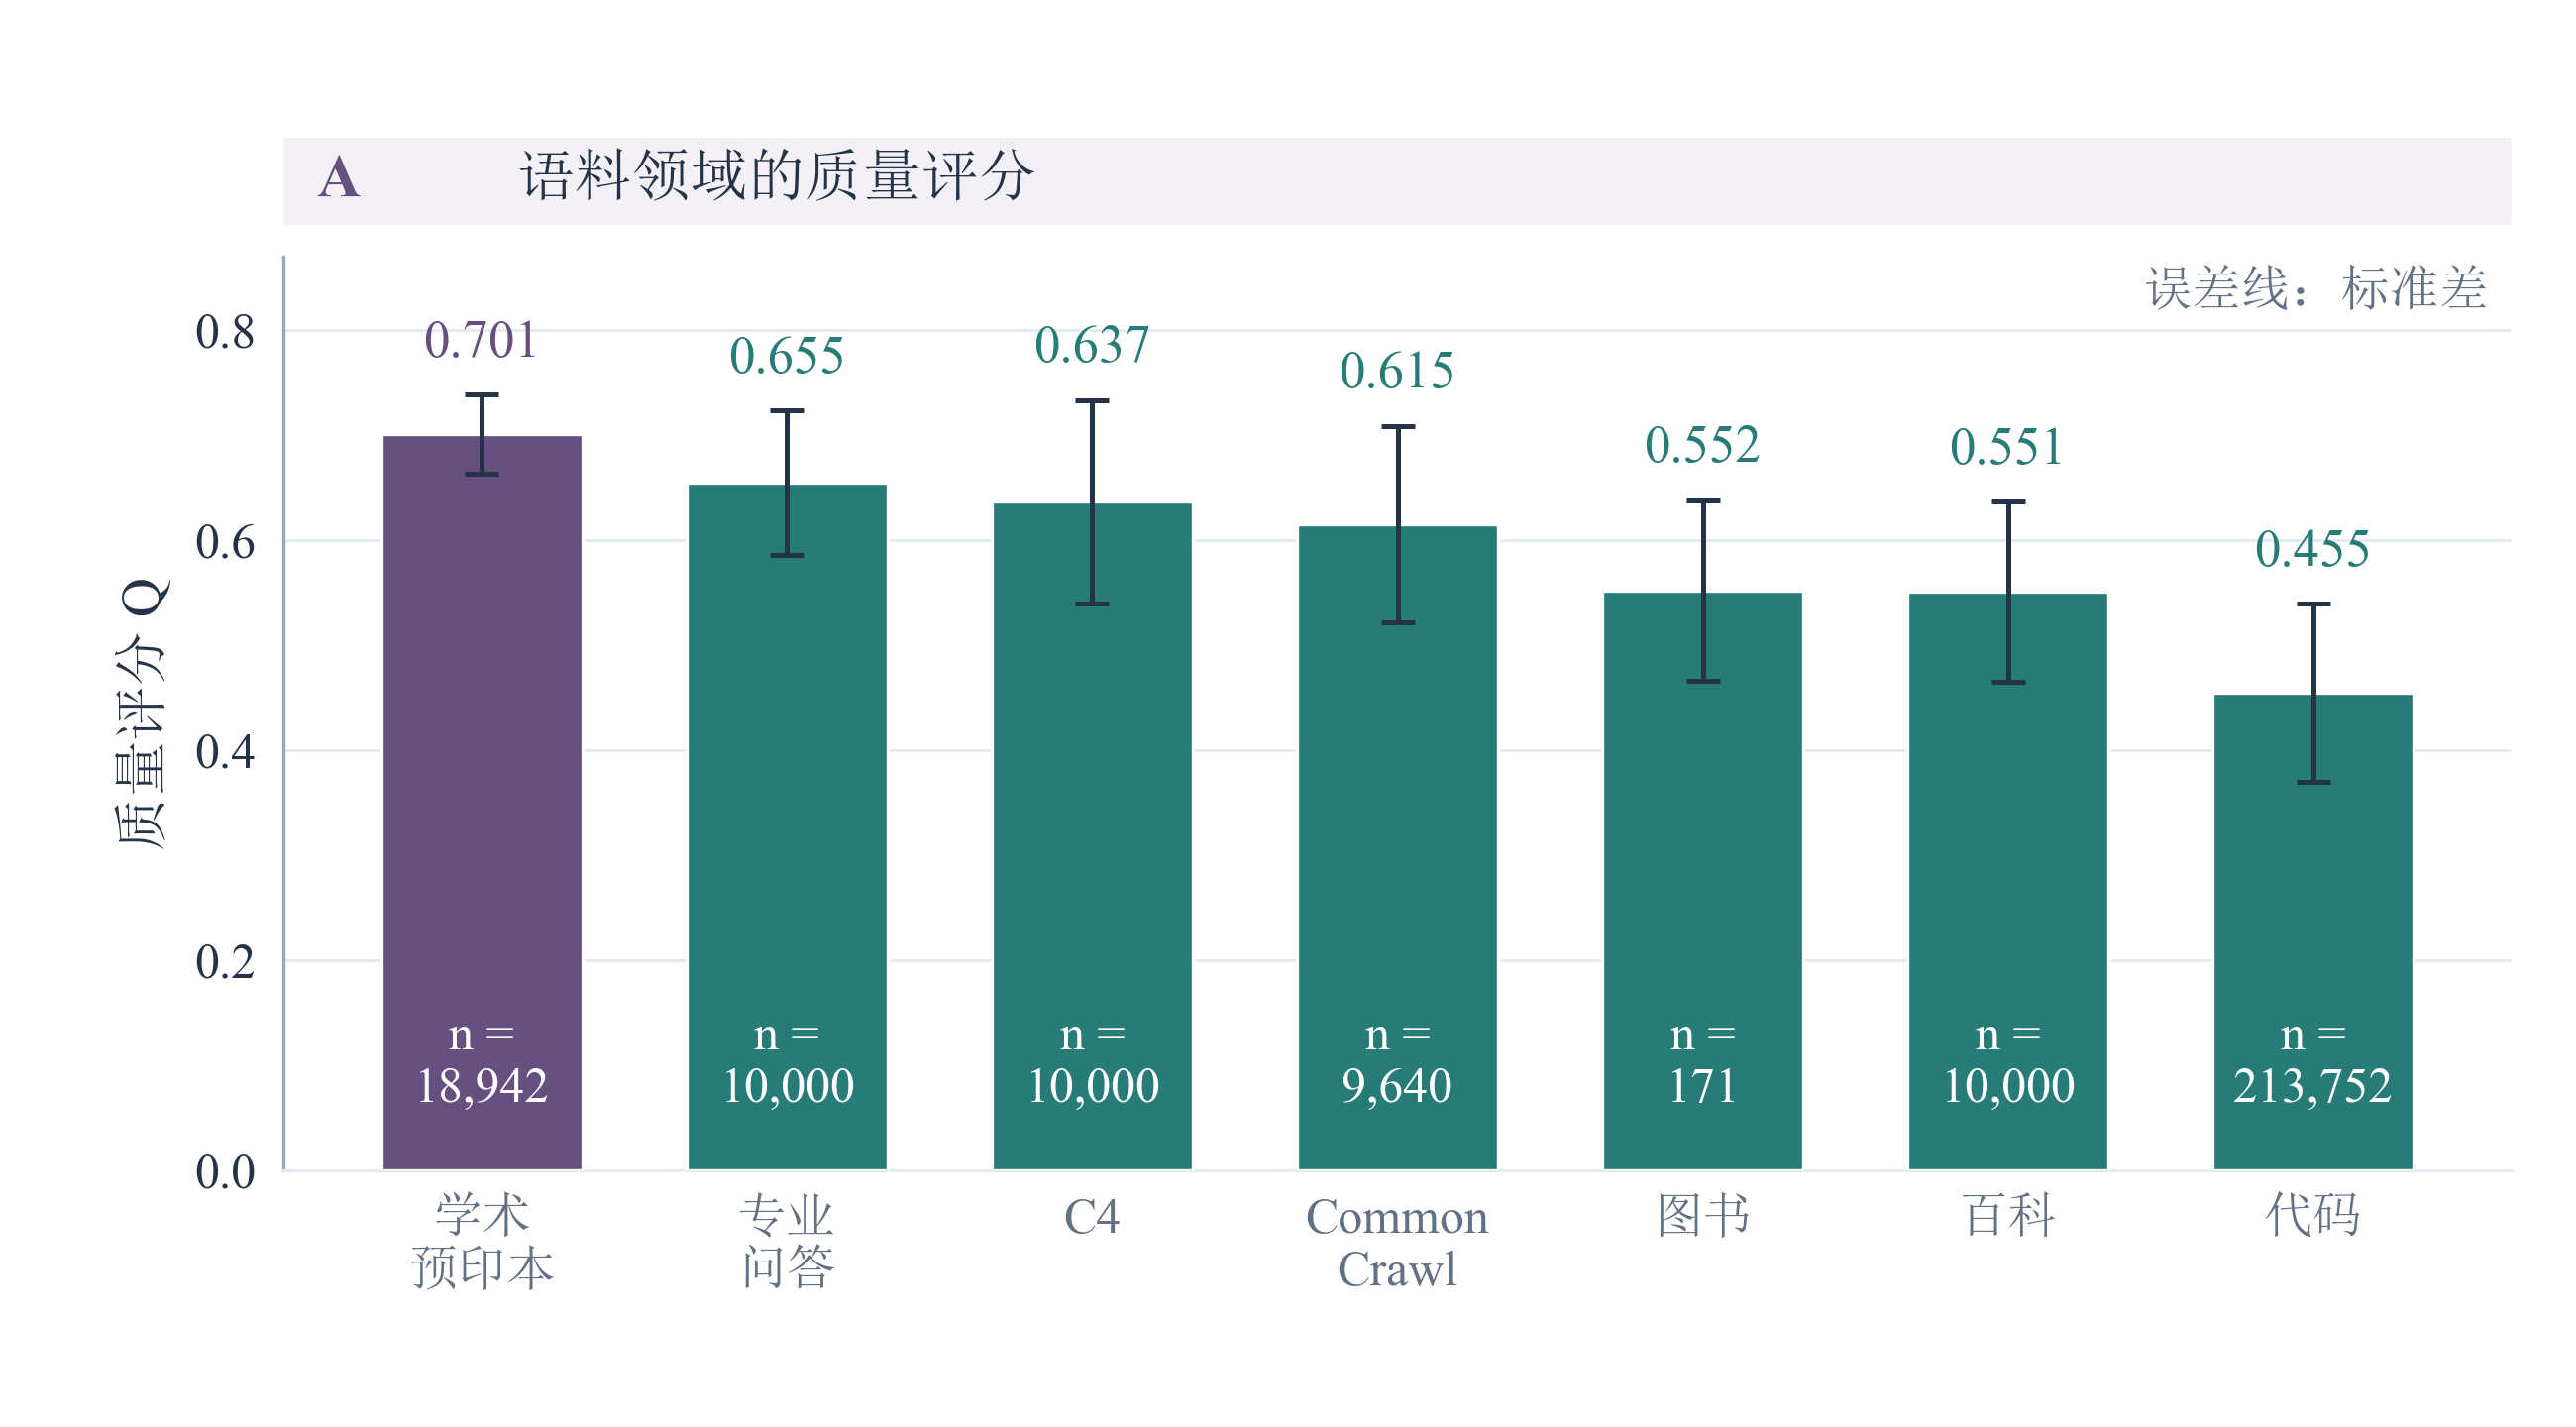
\includegraphics[width=0.62\textwidth]{../求解/问题一/图片/图0_A1-A3全量质量评分.png}
  \caption{A1--A3 全量质量信号的领域级评分（均值±标准差）}
  \label{fig:p1_quality_full}
\end{figure}

\begingroup
\setlength{\tabcolsep}{3pt}
\begin{longtable}{@{}>{\centering\arraybackslash}p{0.20\textwidth}>{\centering\arraybackslash}p{0.16\textwidth}>{\centering\arraybackslash}p{0.16\textwidth}>{\centering\arraybackslash}p{0.16\textwidth}>{\raggedright\arraybackslash}p{0.24\textwidth}@{}}
  \caption{各领域在 A1 抽样集与 A2/A3 扩展集中的质量评分}
  \label{tab:p1_qa} \\
  \toprule
  质量信号领域 & A1 评分 $Q$ & 扩展集评分 $Q$ & 评分差值 & 训练配方对应领域 \\
  \midrule
  \endfirsthead
  \caption{各领域在 A1 抽样集与 A2/A3 扩展集中的质量评分（续）} \\
  \toprule
  质量信号领域 & A1 评分 $Q$ & 扩展集评分 $Q$ & 评分差值 & 训练配方对应领域 \\
  \midrule
  \endhead
  \bottomrule
  \endfoot
  arxiv & 0.7031 & 0.7011 & $+0.0021$ & arxiv \\
  stackexchange & 0.6549 & — & — & stackexchange \\
  c4 & 0.6368 & — & — & （配方侧无同名列） \\
  commoncrawl & 0.6153 & — & — & pile\_\allowbreak{}cc \\
  book & 0.5524 & — & — & gutenberg\_\allowbreak{}pg\_\allowbreak{}19 \\
  wikipedia & 0.5509 & — & — & wikipedia\_\allowbreak{}en \\
  github & 0.4553 & 0.4547 & $+0.0006$ & github \\
\end{longtable}
\endgroup

arxiv 和 github 同时具有抽样与扩展记录，可以直接比较。表\ref{tab:p1_qa}中，两者的评分差分别为 $+0.0021$、$+0.0006$，均接近零。这说明在这两个可比较领域，抽样集和扩展集得到的平均质量较为接近。

全量评分依次为 arxiv（0.703）$>$ stackexchange（0.655）$>$ c4（0.637）$>$ commoncrawl（0.615）$>$ book（0.552）$\approx$ wikipedia（0.551）$>$ github（0.455）。该次序取决于所用的 22 个分类器信号。例如，rps\_\allowbreak{}doc\_\allowbreak{}frac\_\allowbreak{}unique\_\allowbreak{}words 和 rps\_\allowbreak{}doc\_\allowbreak{}unigram\_\allowbreak{}entropy 还会受到文档长度影响。因此，c4、commoncrawl 的评分高于 book、wikipedia，只能说明它们在本评价体系中的得分较高，不能据此判断所有训练任务中的语料价值。

表\ref{tab:p1_conf}比较各集合的冲突比例和排序一致性；图\ref{fig:p1_conf}则给出分歧较多的指标对及对应的熵权分布。

\begingroup
\setlength{\tabcolsep}{3pt}
\begin{longtable}{@{}>{\centering\arraybackslash}p{0.18\textwidth}>{\centering\arraybackslash}p{0.13\textwidth}>{\centering\arraybackslash}p{0.13\textwidth}>{\centering\arraybackslash}p{0.13\textwidth}>{\centering\arraybackslash}p{0.14\textwidth}>{\raggedright\arraybackslash}p{0.20\textwidth}@{}}
  \caption{各数据集的指标冲突比例与排序一致性}
  \label{tab:p1_conf} \\
  \toprule
  统计范围 & 记录数 & Kendall $W$ & 冲突比例 $\rho_c$ & 独立基准 $\rho_0$ & $\rho_c/\rho_0$ \\
  \midrule
  \endfirsthead
  \caption{各数据集的指标冲突比例与排序一致性（续）} \\
  \toprule
  统计范围 & 记录数 & Kendall $W$ & 冲突比例 $\rho_c$ & 独立基准 $\rho_0$ & $\rho_c/\rho_0$ \\
  \midrule
  \endhead
  \bottomrule
  \endfoot
  A1 抽样集 & 51{,}230 & 0.0783 & 0.2252 & 0.2888 & 0.780 \\
  A2+A3 扩展集 & 221{,}275 & 0.0628 & 0.2208 & 0.2888 & 0.764 \\
  全量 & 272{,}505 & 0.0687 & 0.2235 & 0.2888 & 0.774 \\
\end{longtable}
\endgroup

\begin{figure}[ht]
  \centering
  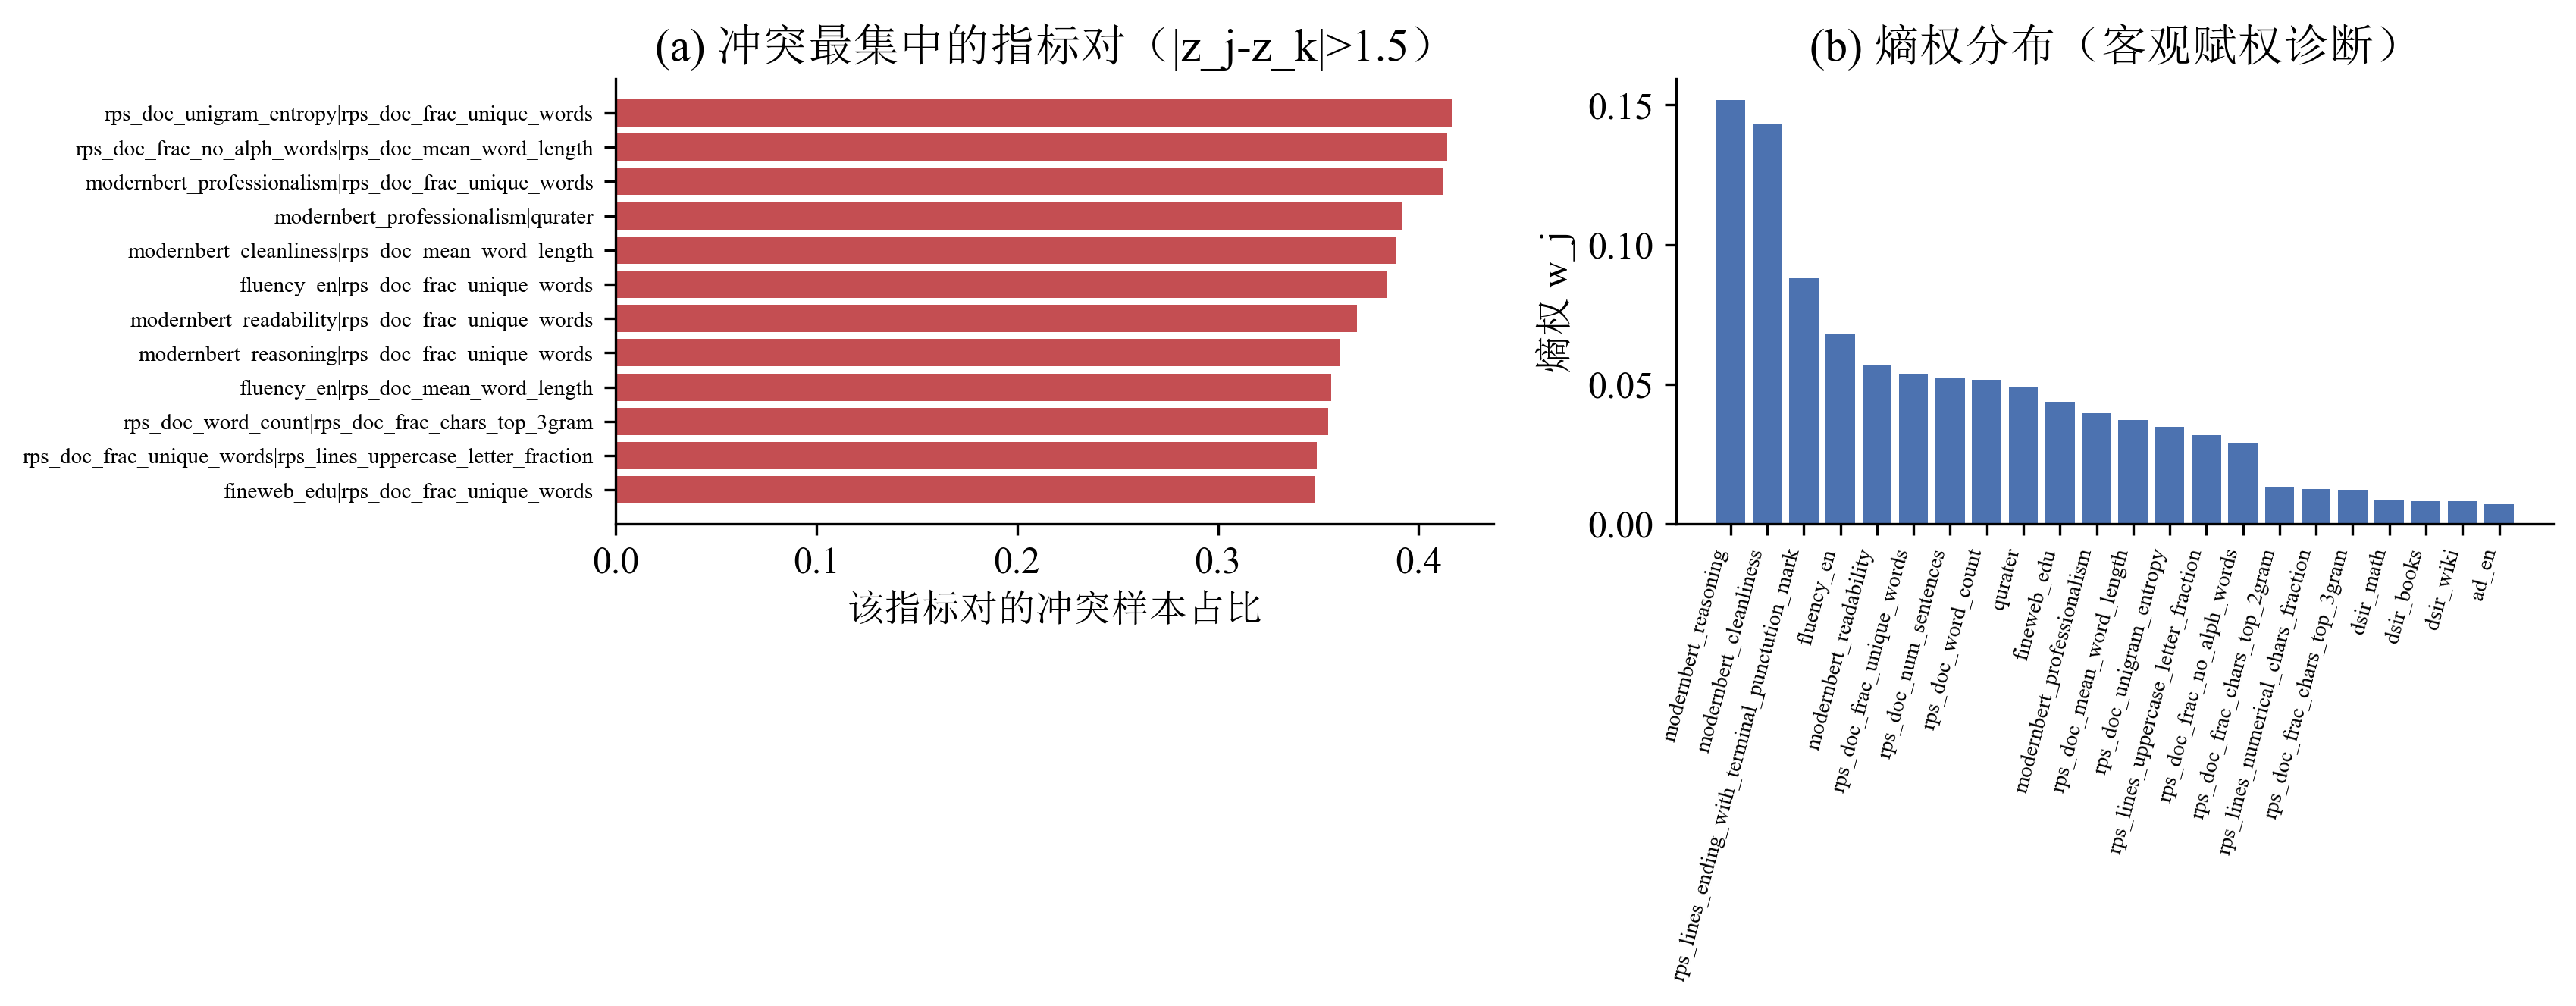
\includegraphics[width=0.92\textwidth]{../求解/问题一/图片/图6_冲突与赋权诊断.png}
  \caption{冲突最集中的指标对（左）与熵权分布（右）}
  \label{fig:p1_conf}
\end{figure}

表\ref{tab:p1_conf}中，抽样集、扩展集和全量记录的冲突率都在 $0.221\sim0.225$ 之间，表明更换统计集合后，冲突比例变化较小。

全量 Kendall 系数为 $0.069$，说明指标排序的一致程度较弱。虽然 $\chi^2$ 检验得到 $p<0.001$，但样本量很大，统计显著并不等于高度一致。同时，$22.3\%$ 的冲突率低于独立参照的 $28.9\%$，比值为 $0.774$。两项结果合起来看，各指标存在共同倾向，但仍保留较多评价分歧。

结合字段含义，可从三方面理解这些分歧。首先，指标的具体测量方式不同，如 rps\_\allowbreak{}doc\_\allowbreak{}unigram\_\allowbreak{}entropy 与 rps\_\allowbreak{}doc\_\allowbreak{}frac\_\allowbreak{}unique\_\allowbreak{}words 虽都涉及词汇多样性，计算尺度却不同。其次，同一指标在不同内容上可能有不同表现，例如 modernbert\_\allowbreak{}professionalism 对学术文本和论坛文本的评价。最后，分布形态也有影响，ad\_\allowbreak{}en 的二分类概率在长文档上容易集中于两端。

处理时保留这些样本参与领域均值计算，同时按 $Q_i$ 相对领域中位数的位置作综合裁决，并保留冲突标记。问题二、三使用聚合结果，不将冲突样本单独作为分析依据。

\Needspace{4\baselineskip}
\textbf{2. 领域配比与损失的拟合及验证}\par\nopagebreak[4]

配比拟合的结果从四个角度展示：图\ref{fig:p1_structure}给出训练配方构成，图\ref{fig:p1_r2}比较训练与检验精度，图\ref{fig:p1_scatter}对照同尺度的预测和观测损失，图\ref{fig:p1_heatmap}展示不同训练领域的系数差异。

\begin{figure}[ht]
  \centering
  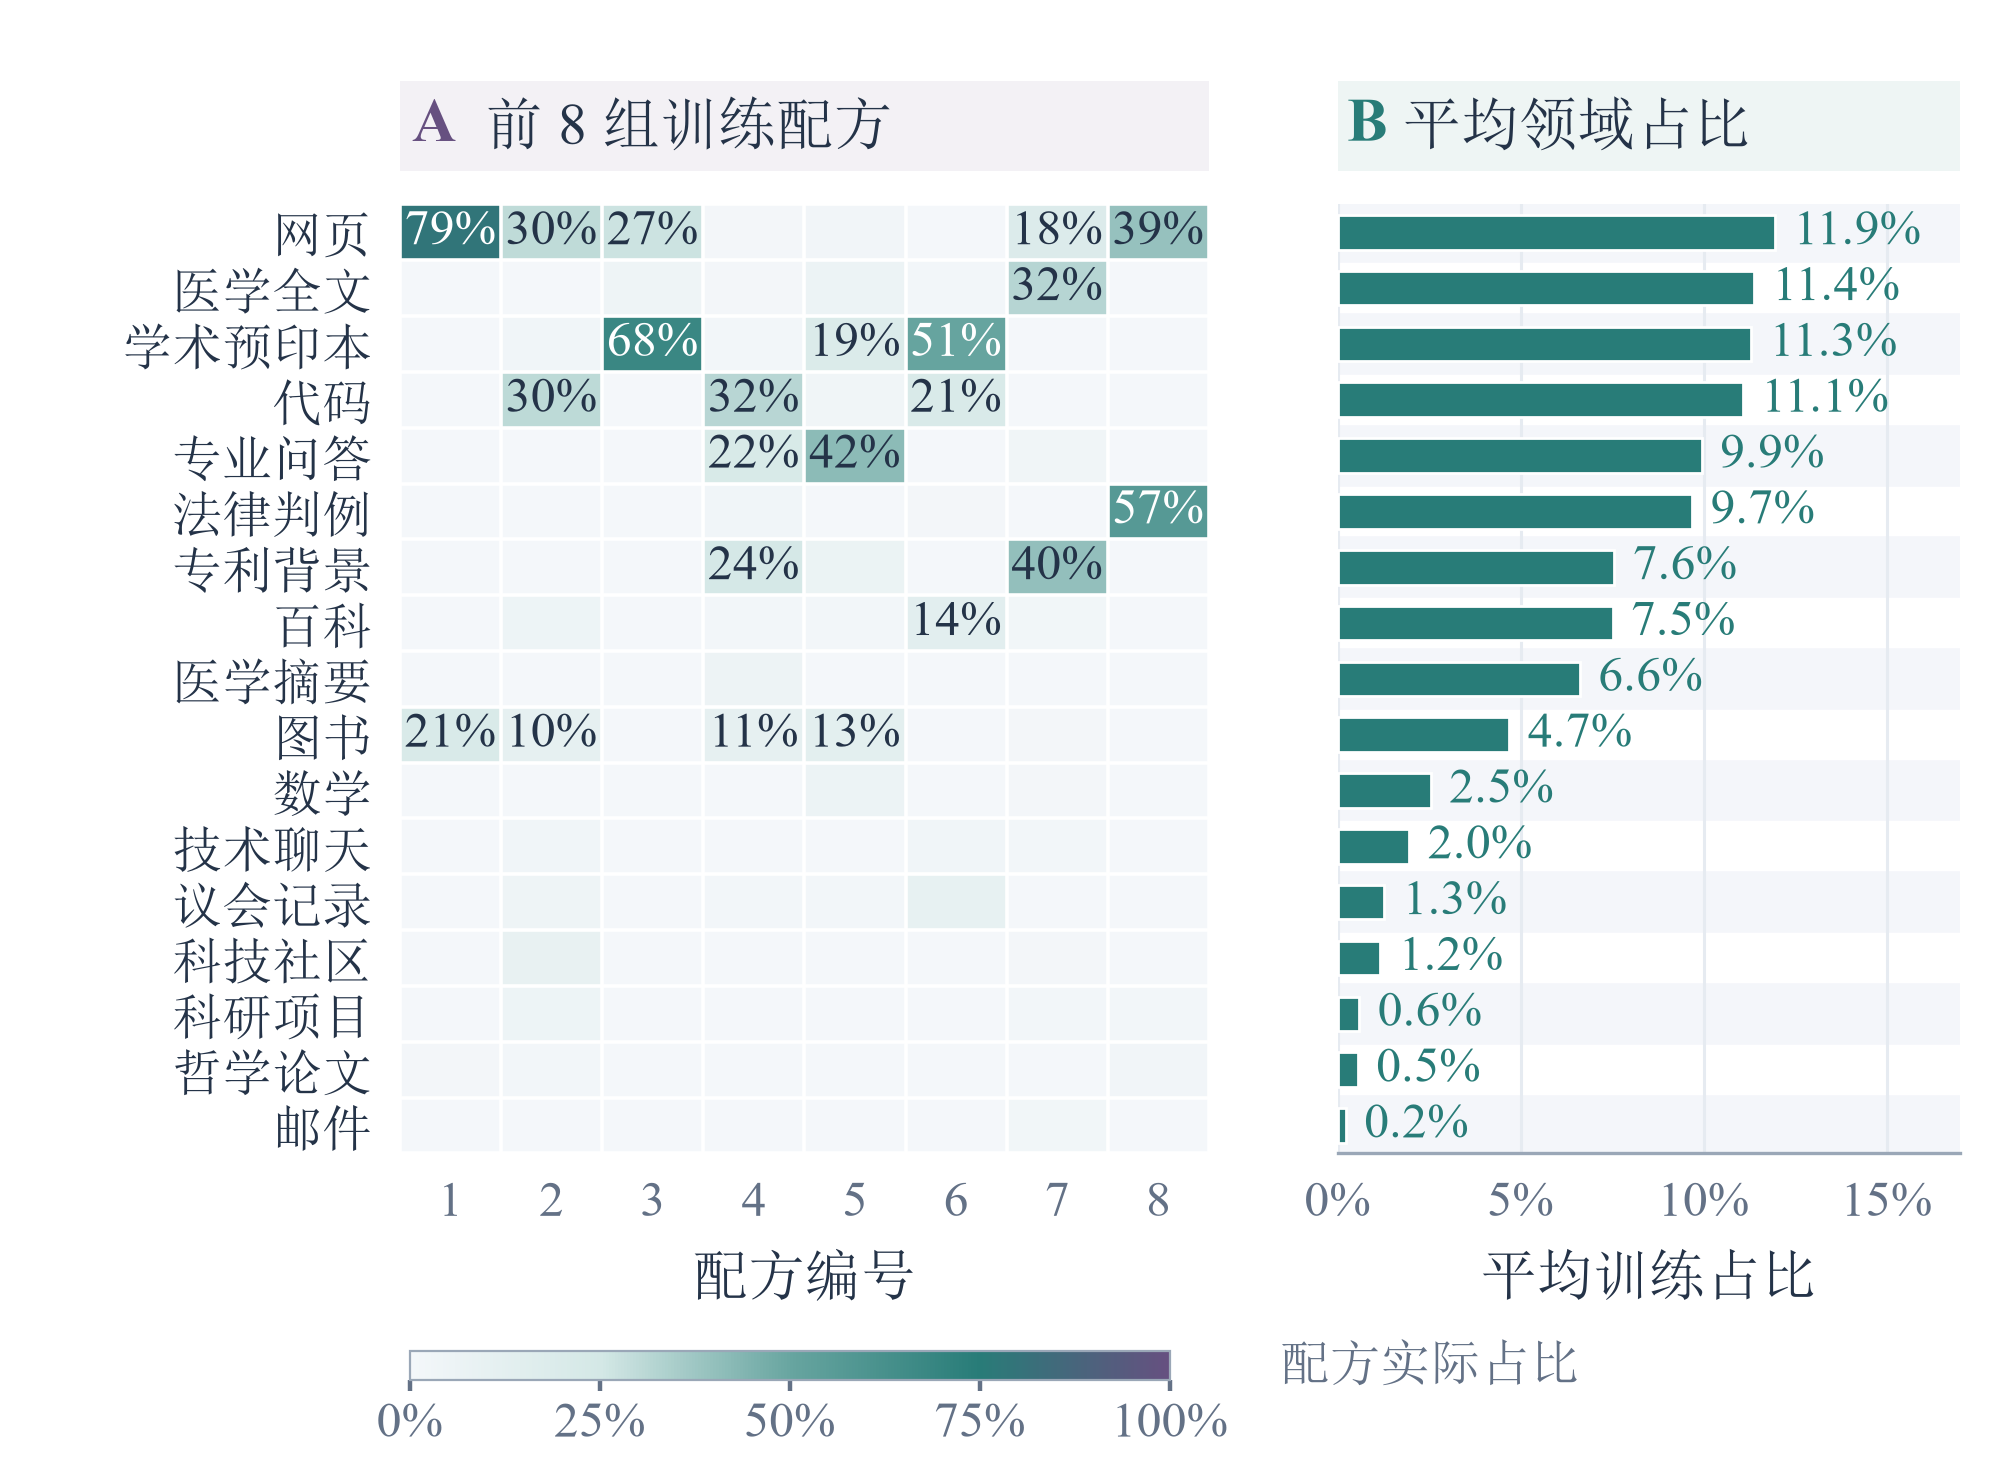
\includegraphics[width=0.92\textwidth]{../求解/问题一/图片/图1_训练配比结构.png}
  \caption{训练配方结构（左：前 8 组配方堆叠；右：全部配方平均配比）}
  \label{fig:p1_structure}
\end{figure}

\begin{figure}[ht]
  \centering
  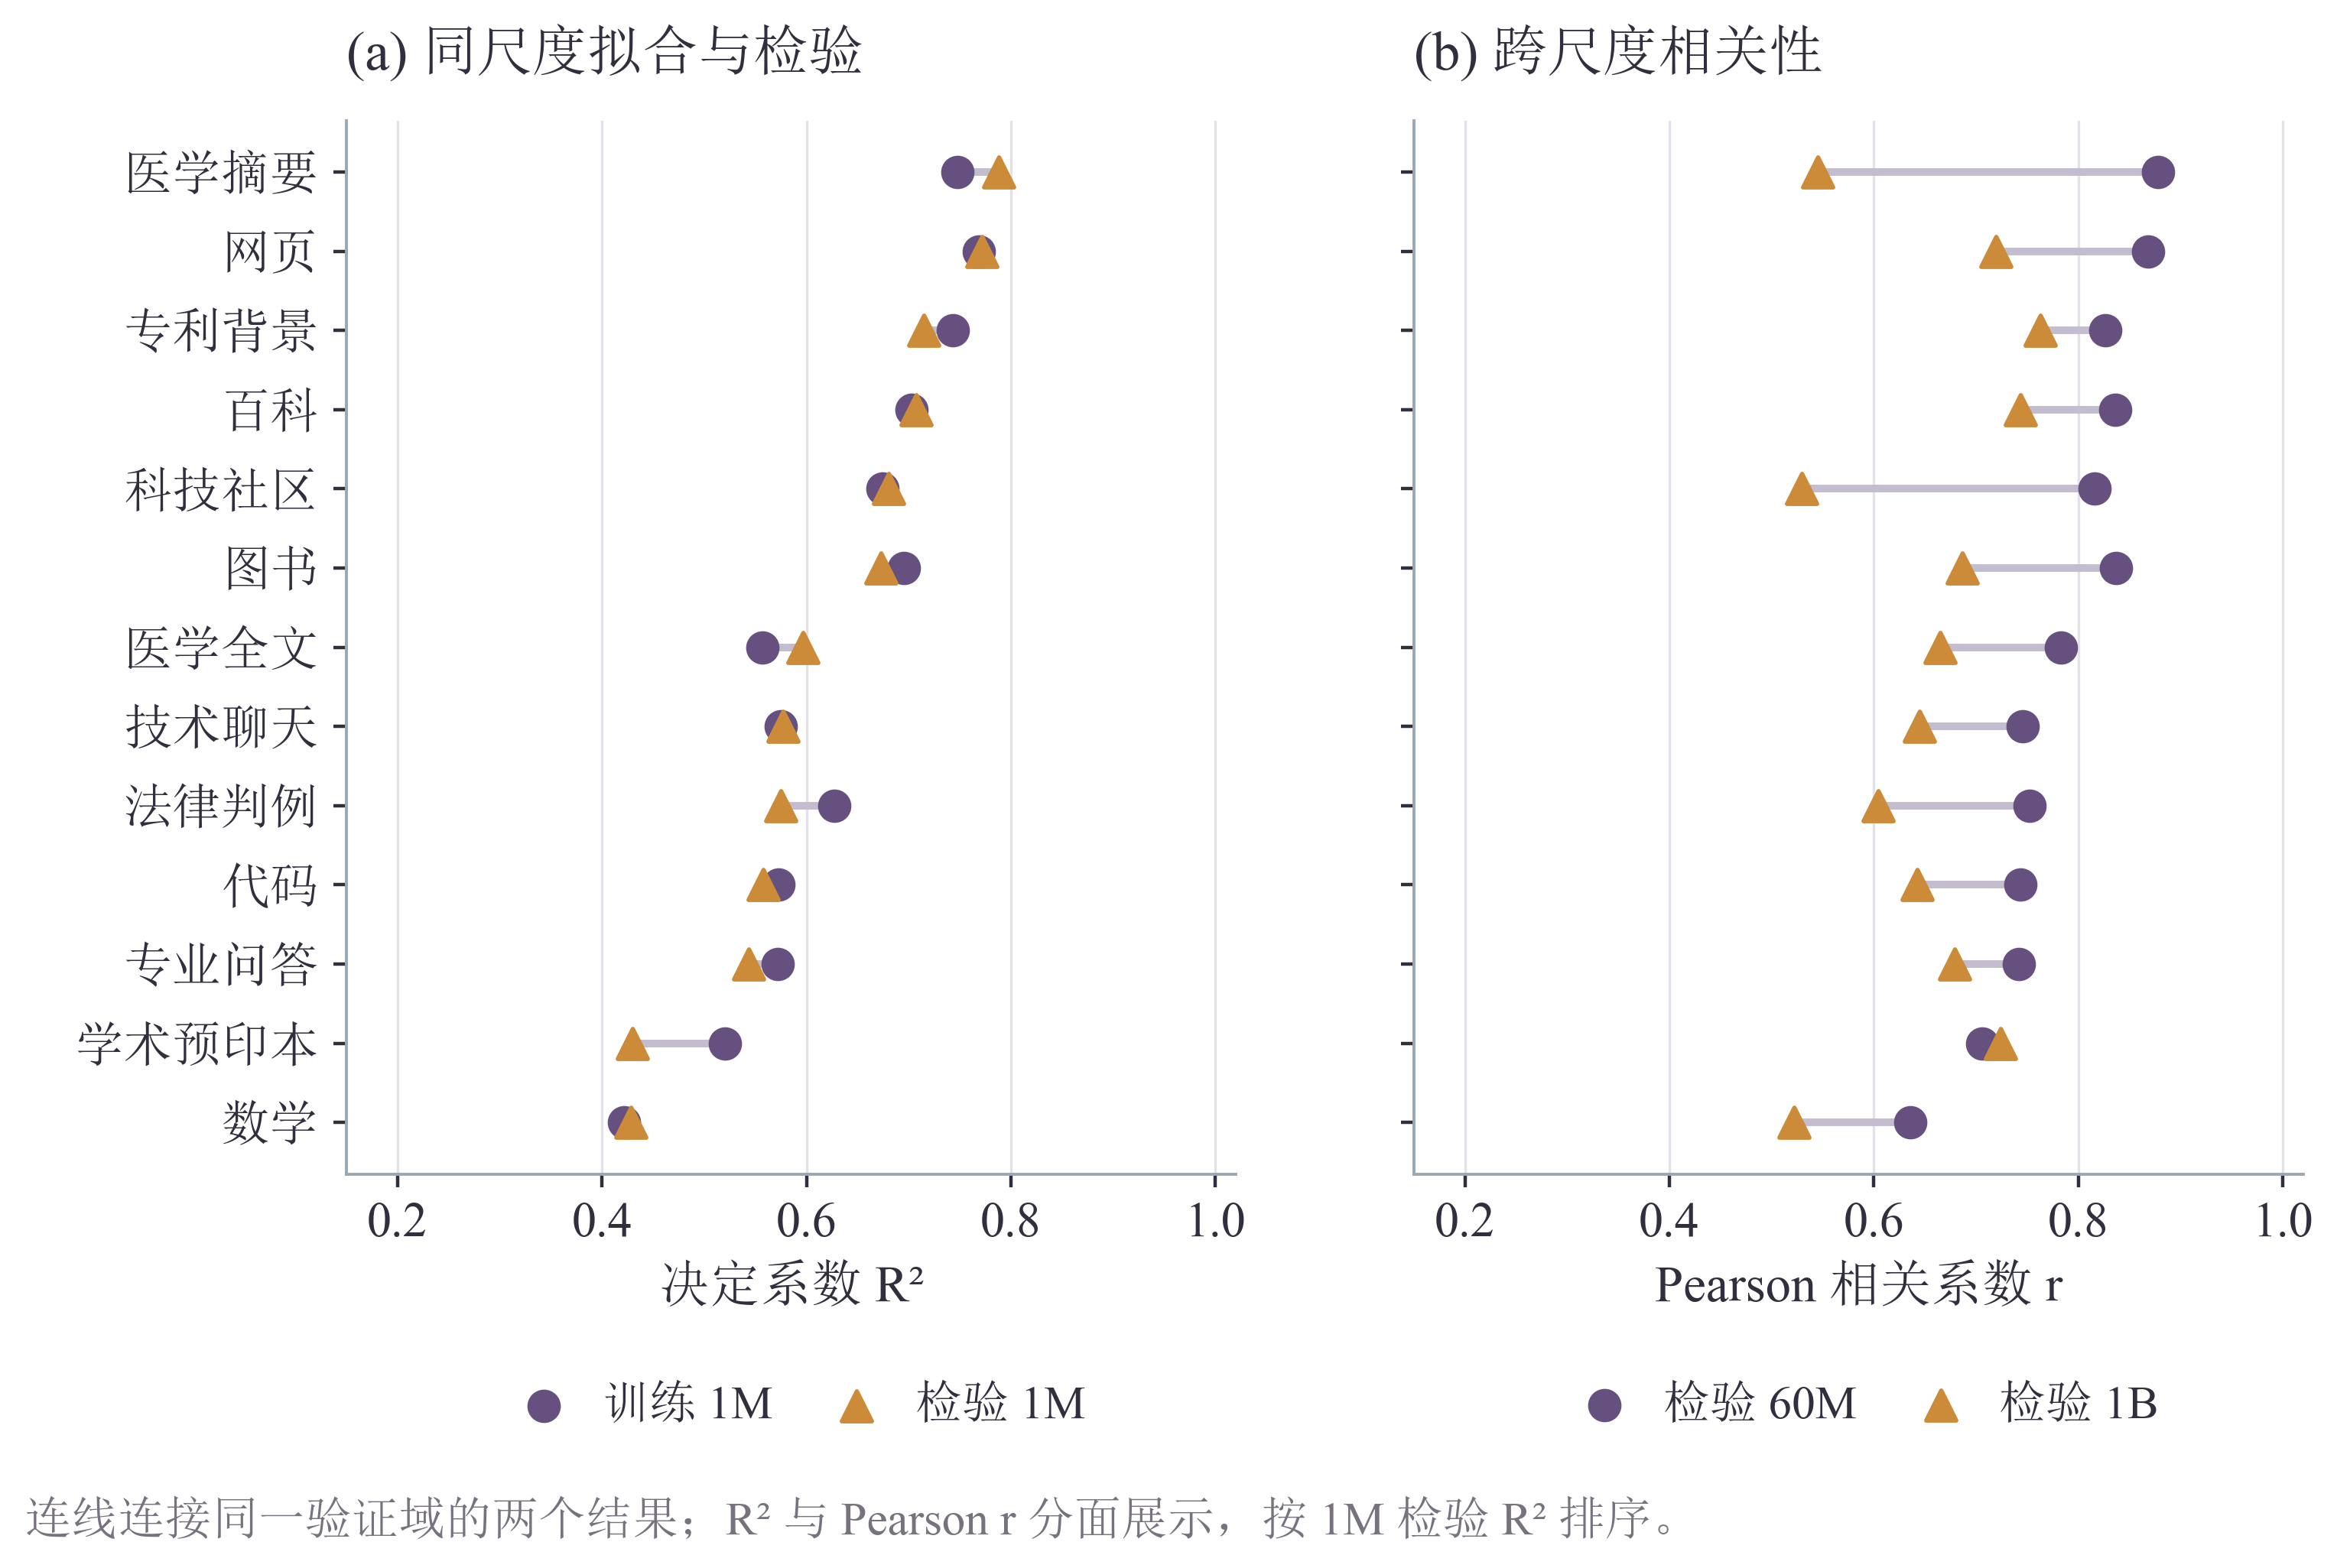
\includegraphics[width=0.72\textwidth]{../求解/问题一/图片/图2_线性模型R2.png}
  \caption{线性混合回归的拟合与泛化表现}
  \label{fig:p1_r2}
\end{figure}

\begin{figure}[ht]
  \centering
  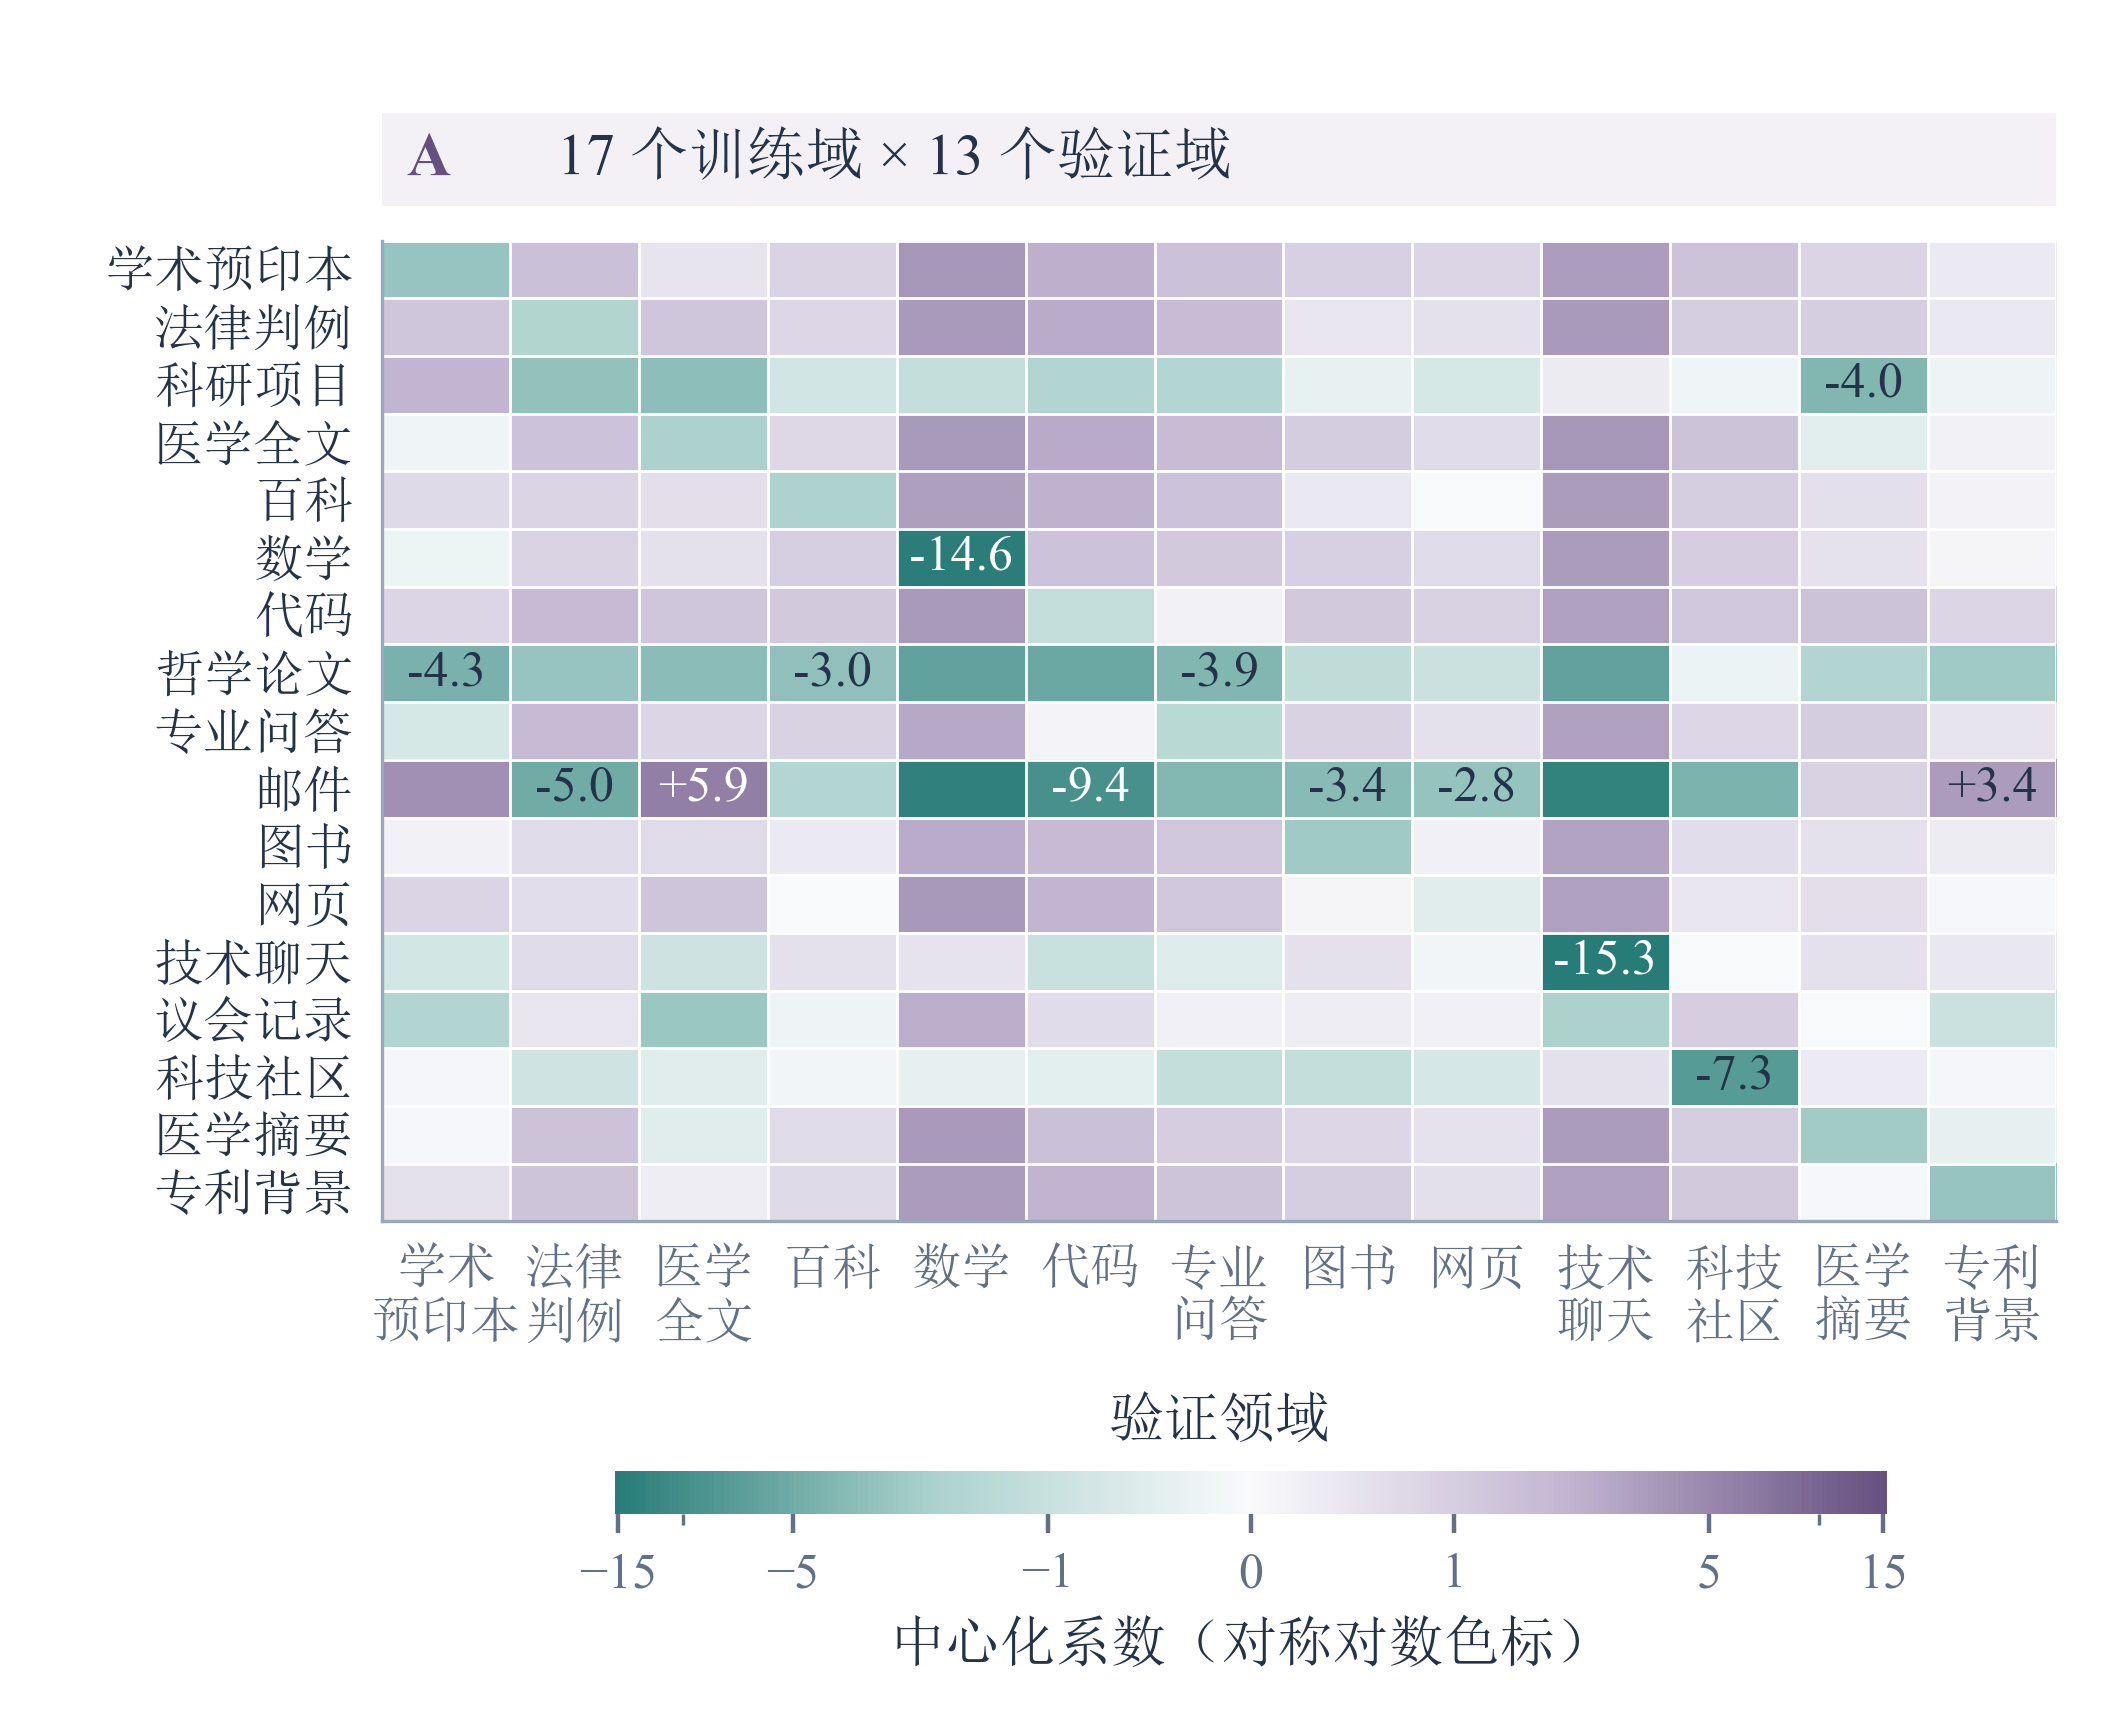
\includegraphics[width=0.78\textwidth]{../求解/问题一/图片/图4_混合系数热力图.png}
  \caption{领域配比对交叉熵损失的相对影响热力图}
  \label{fig:p1_heatmap}
\end{figure}

\begin{figure}[ht]
  \centering
  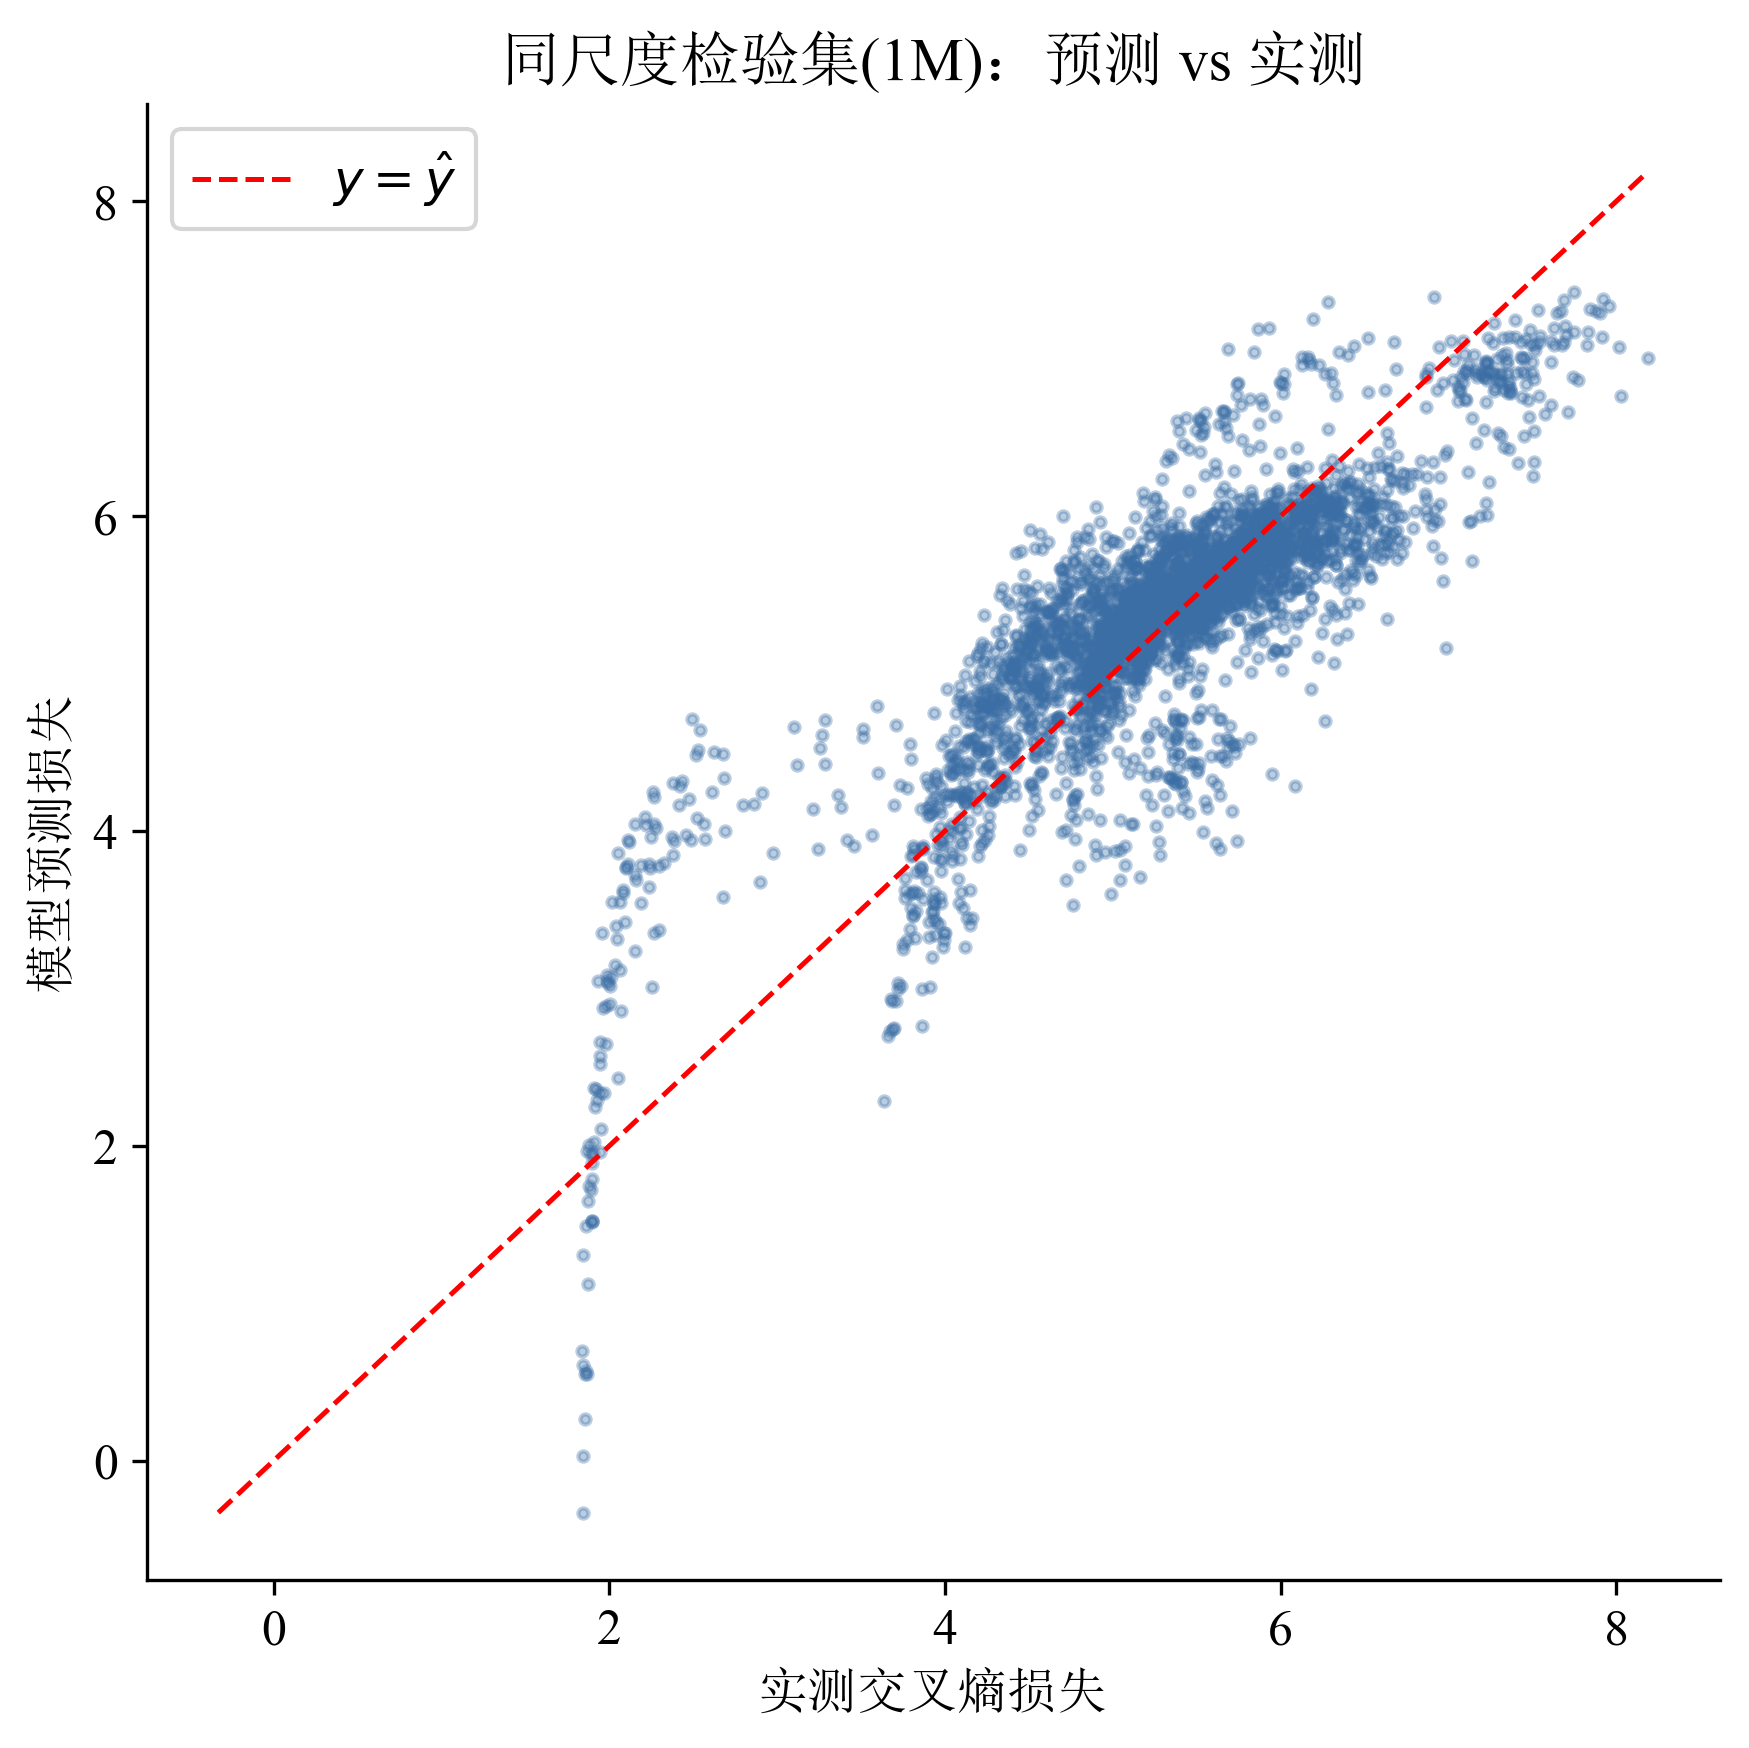
\includegraphics[width=0.58\textwidth]{../求解/问题一/图片/图3_预测vs实测.png}
  \caption{同尺度检验集（1M）预测损失与实测损失对比}
  \label{fig:p1_scatter}
\end{figure}

在图\ref{fig:p1_r2}中，13 个验证域的训练 $R^2$ 为 $0.42\sim0.77$，平均为 $0.629$。1M 同尺度检验的平均值为 $0.619$，与训练结果接近，未显示明显的训练集过拟合现象。

不同规模模型的损失基准不同，60M 与 1M 的损失比约为 $0.68$，直接沿用原损失尺度会影响误差评价。为比较变化趋势，我们补充计算 Pearson 相关：60M 和 1B 检验集的平均值分别为 $0.782$、$0.651$。这支持配比关系在跨规模时仍保留部分预测趋势，但绝对损失还需考虑尺度调整。

图\ref{fig:p1_heatmap}显示，各训练领域对验证任务的作用并不相同。dm\_\allowbreak{}mathematics、arxiv 等领域在部分任务上对应较低损失，pile\_\allowbreak{}cc、ubuntu\_\allowbreak{}irc 等领域则表现出不同方向。配比选择因而需要结合验证任务权重，不能仅看某一个系数。

在原模型中再加入混合质量指数 $\bar Q$ 后，13 个验证域的平均 $R^2$ 仅提高 $9.9\times10^{-5}$。由于 $\bar Q$ 本身由配比线性组合而成，这一结果说明它在当前模型中没有提供明显的新信息。本文因此保留原配比回归，并在问题二、三中通过附件 B 的半合成质量实验讨论质量投入。

文本质量与损失难度并非同一个概念。图\ref{fig:p1_quality}利用 6 个可映射领域，对照 A1--A3 的熵权评分 $Q$ 与损失代理 $Q^{(\text{loss})}$ 的排序。

\begin{figure}[ht]
  \centering
  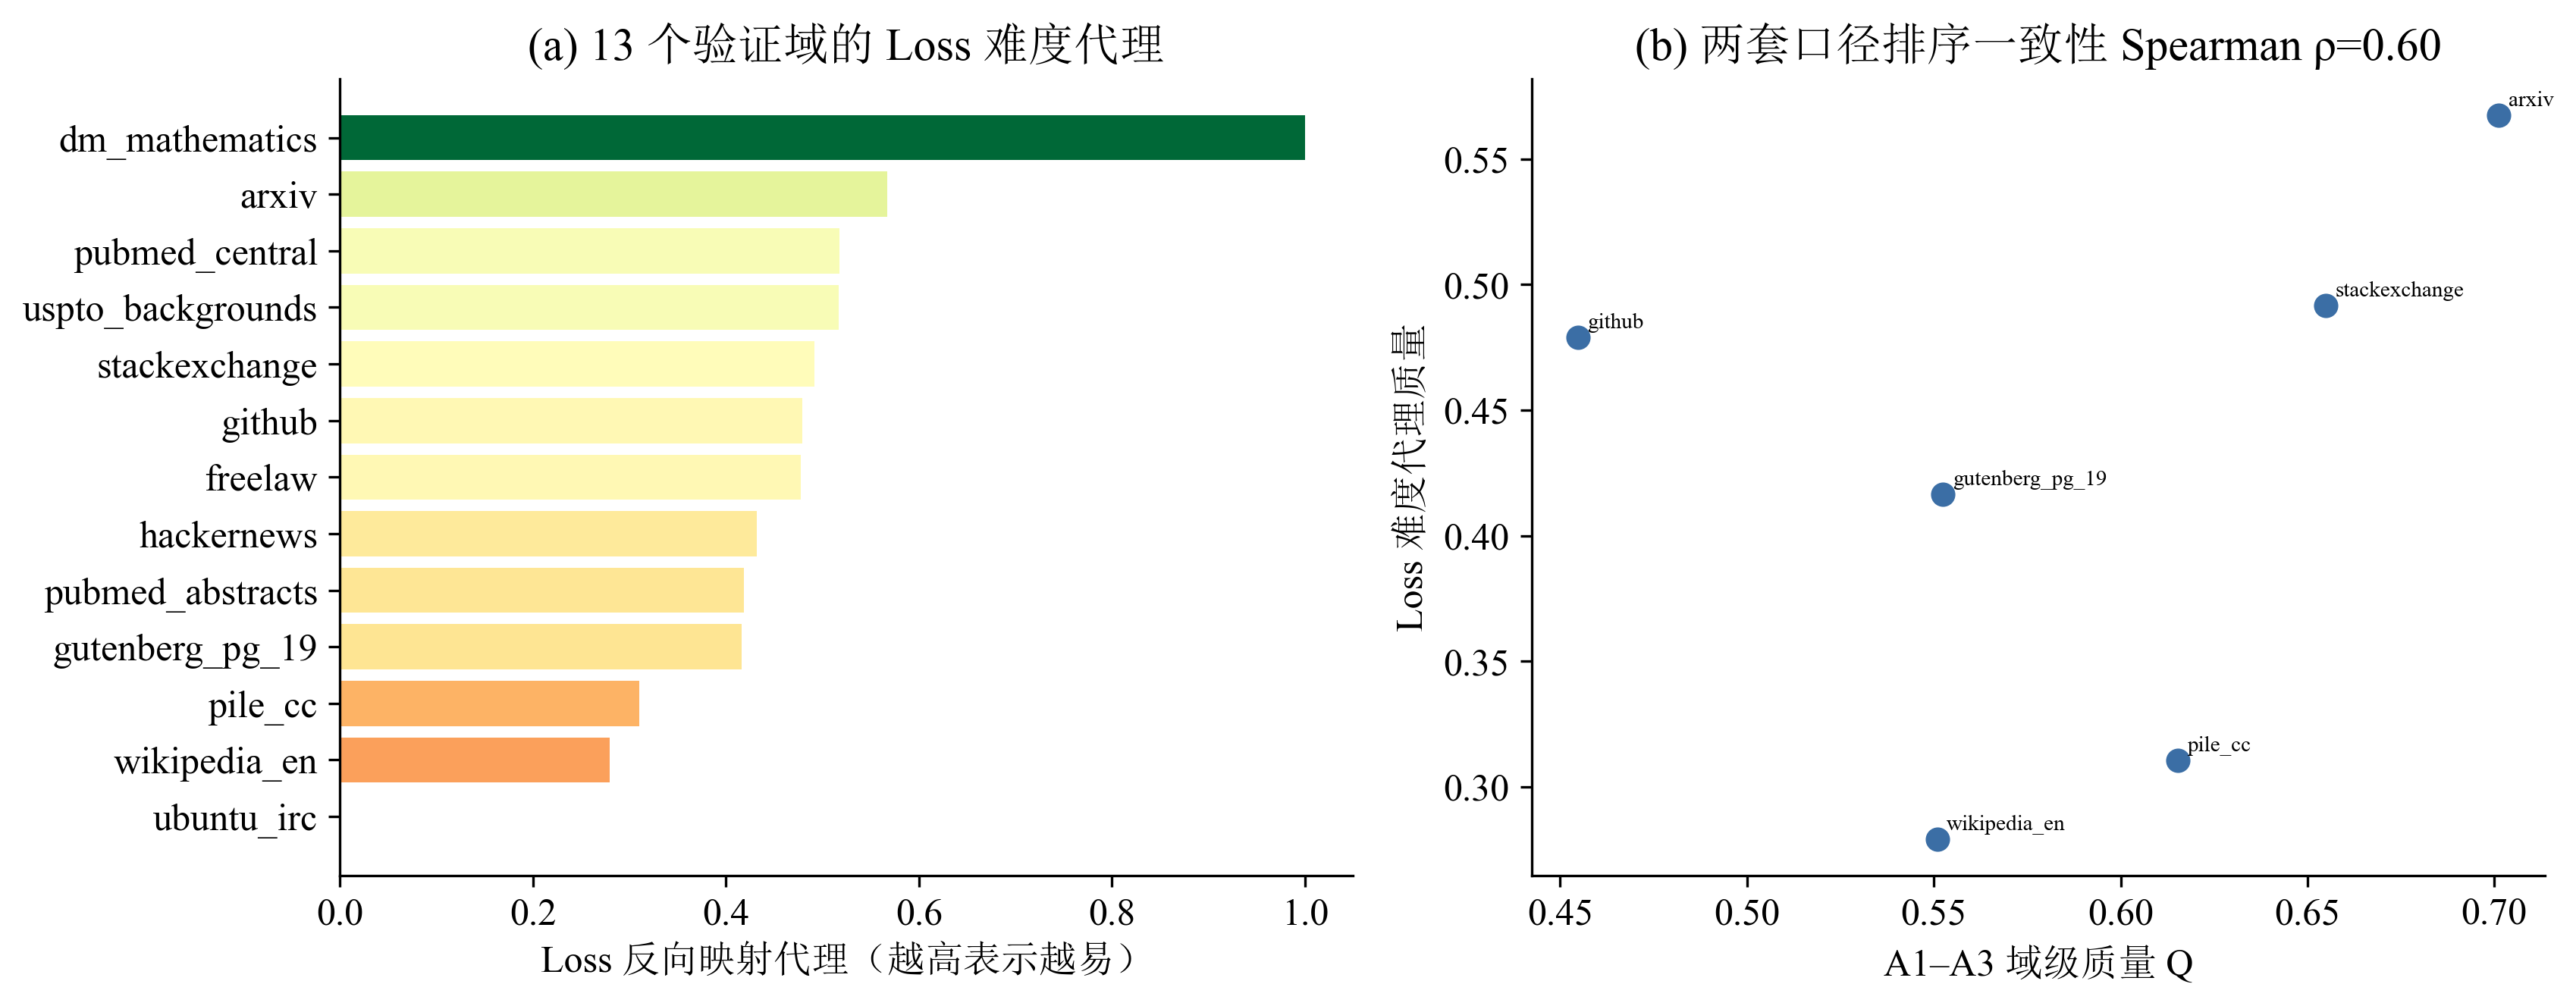
\includegraphics[width=0.92\textwidth]{../求解/问题一/图片/图5_领域质量评分.png}
  \caption{左：13 个验证域的损失难度代理；右：A1--A3 质量与损失难度代理的排序一致性}
  \label{fig:p1_quality}
\end{figure}

图\ref{fig:p1_quality}(a)比较了 13 个验证域，其中 dm\_\allowbreak{}mathematics 的代理质量为 $1.000$，ubuntu\_\allowbreak{}irc 为 $0.000$，分别对应本组验证损失的低端和高端。图\ref{fig:p1_quality}(b)所用 direct/near\_\allowbreak{}direct 映射来自 A16，两套评分的 Spearman 系数为 $0.60$。arxiv、stackexchange、github 的相对次序较一致，而 wikipedia、book、pile\_\allowbreak{}cc 存在分歧。这说明文本被评为高质量，并不保证在当前模型和验证条件下容易拟合。后续进行语料治理时采用文本质量评分，预测损失时则另行考虑领域难度。

\Needspace{4\baselineskip}
\textbf{3. 配比推荐与跨尺度分析}\par\nopagebreak[4]

若不限制各域占比上限，线性目标会将配方集中到单一低损失领域，预测加权损失为 $4.177$。为避免推荐方案过度集中，本文把上限设为参考占比的 2.5 倍。表\ref{tab:p1_rec}给出的有界方案使预测损失从 $5.336$ 降至 $5.136$，按未舍入结果计算下降 $0.199$。

\begingroup
\setlength{\tabcolsep}{3pt}
\begin{longtable}{@{}>{\centering\arraybackslash}p{0.30\textwidth}>{\centering\arraybackslash}p{0.22\textwidth}>{\centering\arraybackslash}p{0.22\textwidth}>{\centering\arraybackslash}p{0.20\textwidth}@{}}
  \caption{配比上限约束下的推荐方案与参考方案}
  \label{tab:p1_rec} \\
  \toprule
  训练领域 & 参考占比 & 推荐占比 & 占比变化量 \\
  \midrule
  \endfirsthead
  \caption{配比上限约束下的推荐方案与参考方案（续）} \\
  \toprule
  训练领域 & 参考占比 & 推荐占比 & 占比变化量 \\
  \midrule
  \endhead
  \bottomrule
  \endfoot
  pubmed\_\allowbreak{}central & 0.1137 & 0.2843 & $+0.1706$ \\
  stackexchange & 0.0994 & 0.2486 & $+0.1491$ \\
  pubmed\_\allowbreak{}abstracts & 0.0662 & 0.1654 & $+0.0993$ \\
  gutenberg\_\allowbreak{}pg\_\allowbreak{}19 & 0.0469 & 0.1173 & $+0.0704$ \\
  dm\_\allowbreak{}mathematics & 0.0255 & 0.0637 & $+0.0382$ \\
  uspto\_\allowbreak{}backgrounds & 0.0755 & 0.0000 & $-0.0755$ \\
  freelaw & 0.0968 & 0.0000 & $-0.0968$ \\
  github & 0.1107 & 0.0000 & $-0.1107$ \\
  arxiv & 0.1130 & 0.0000 & $-0.1130$ \\
  pile\_\allowbreak{}cc & 0.1195 & 0.0000 & $-0.1195$ \\
\end{longtable}
\endgroup

表\ref{tab:p1_rec}中，pubmed\_\allowbreak{}central、stackexchange、pubmed\_\allowbreak{}abstracts 的推荐占比增加，pile\_\allowbreak{}cc、arxiv、github、freelaw 的占比下降。这里优化的是 13 个验证域的加权平均损失，因此结果不等同于各领域自身表现的优劣。例如，arxiv 的占比降低只表示在当前权重和约束下，其他分配更有利于总体目标，不能解释为该领域文本质量低。

图\ref{fig:p1_extrap}进一步比较规模变化后的损失比例。10B 外推表的 est/train 因子均值为 $0.338$、标准差为 $0.038$，70B 对应 $0.266$ 和 $0.036$；同配方下，各域 60M/1M 损失比的均值为 $0.51\sim0.82$。这些比例可作为调整跨规模预测的参照，其中 10B、70B 本身属于外推记录，只能用于检查估算关系的一致性。

\begin{figure}[H]
  \centering
  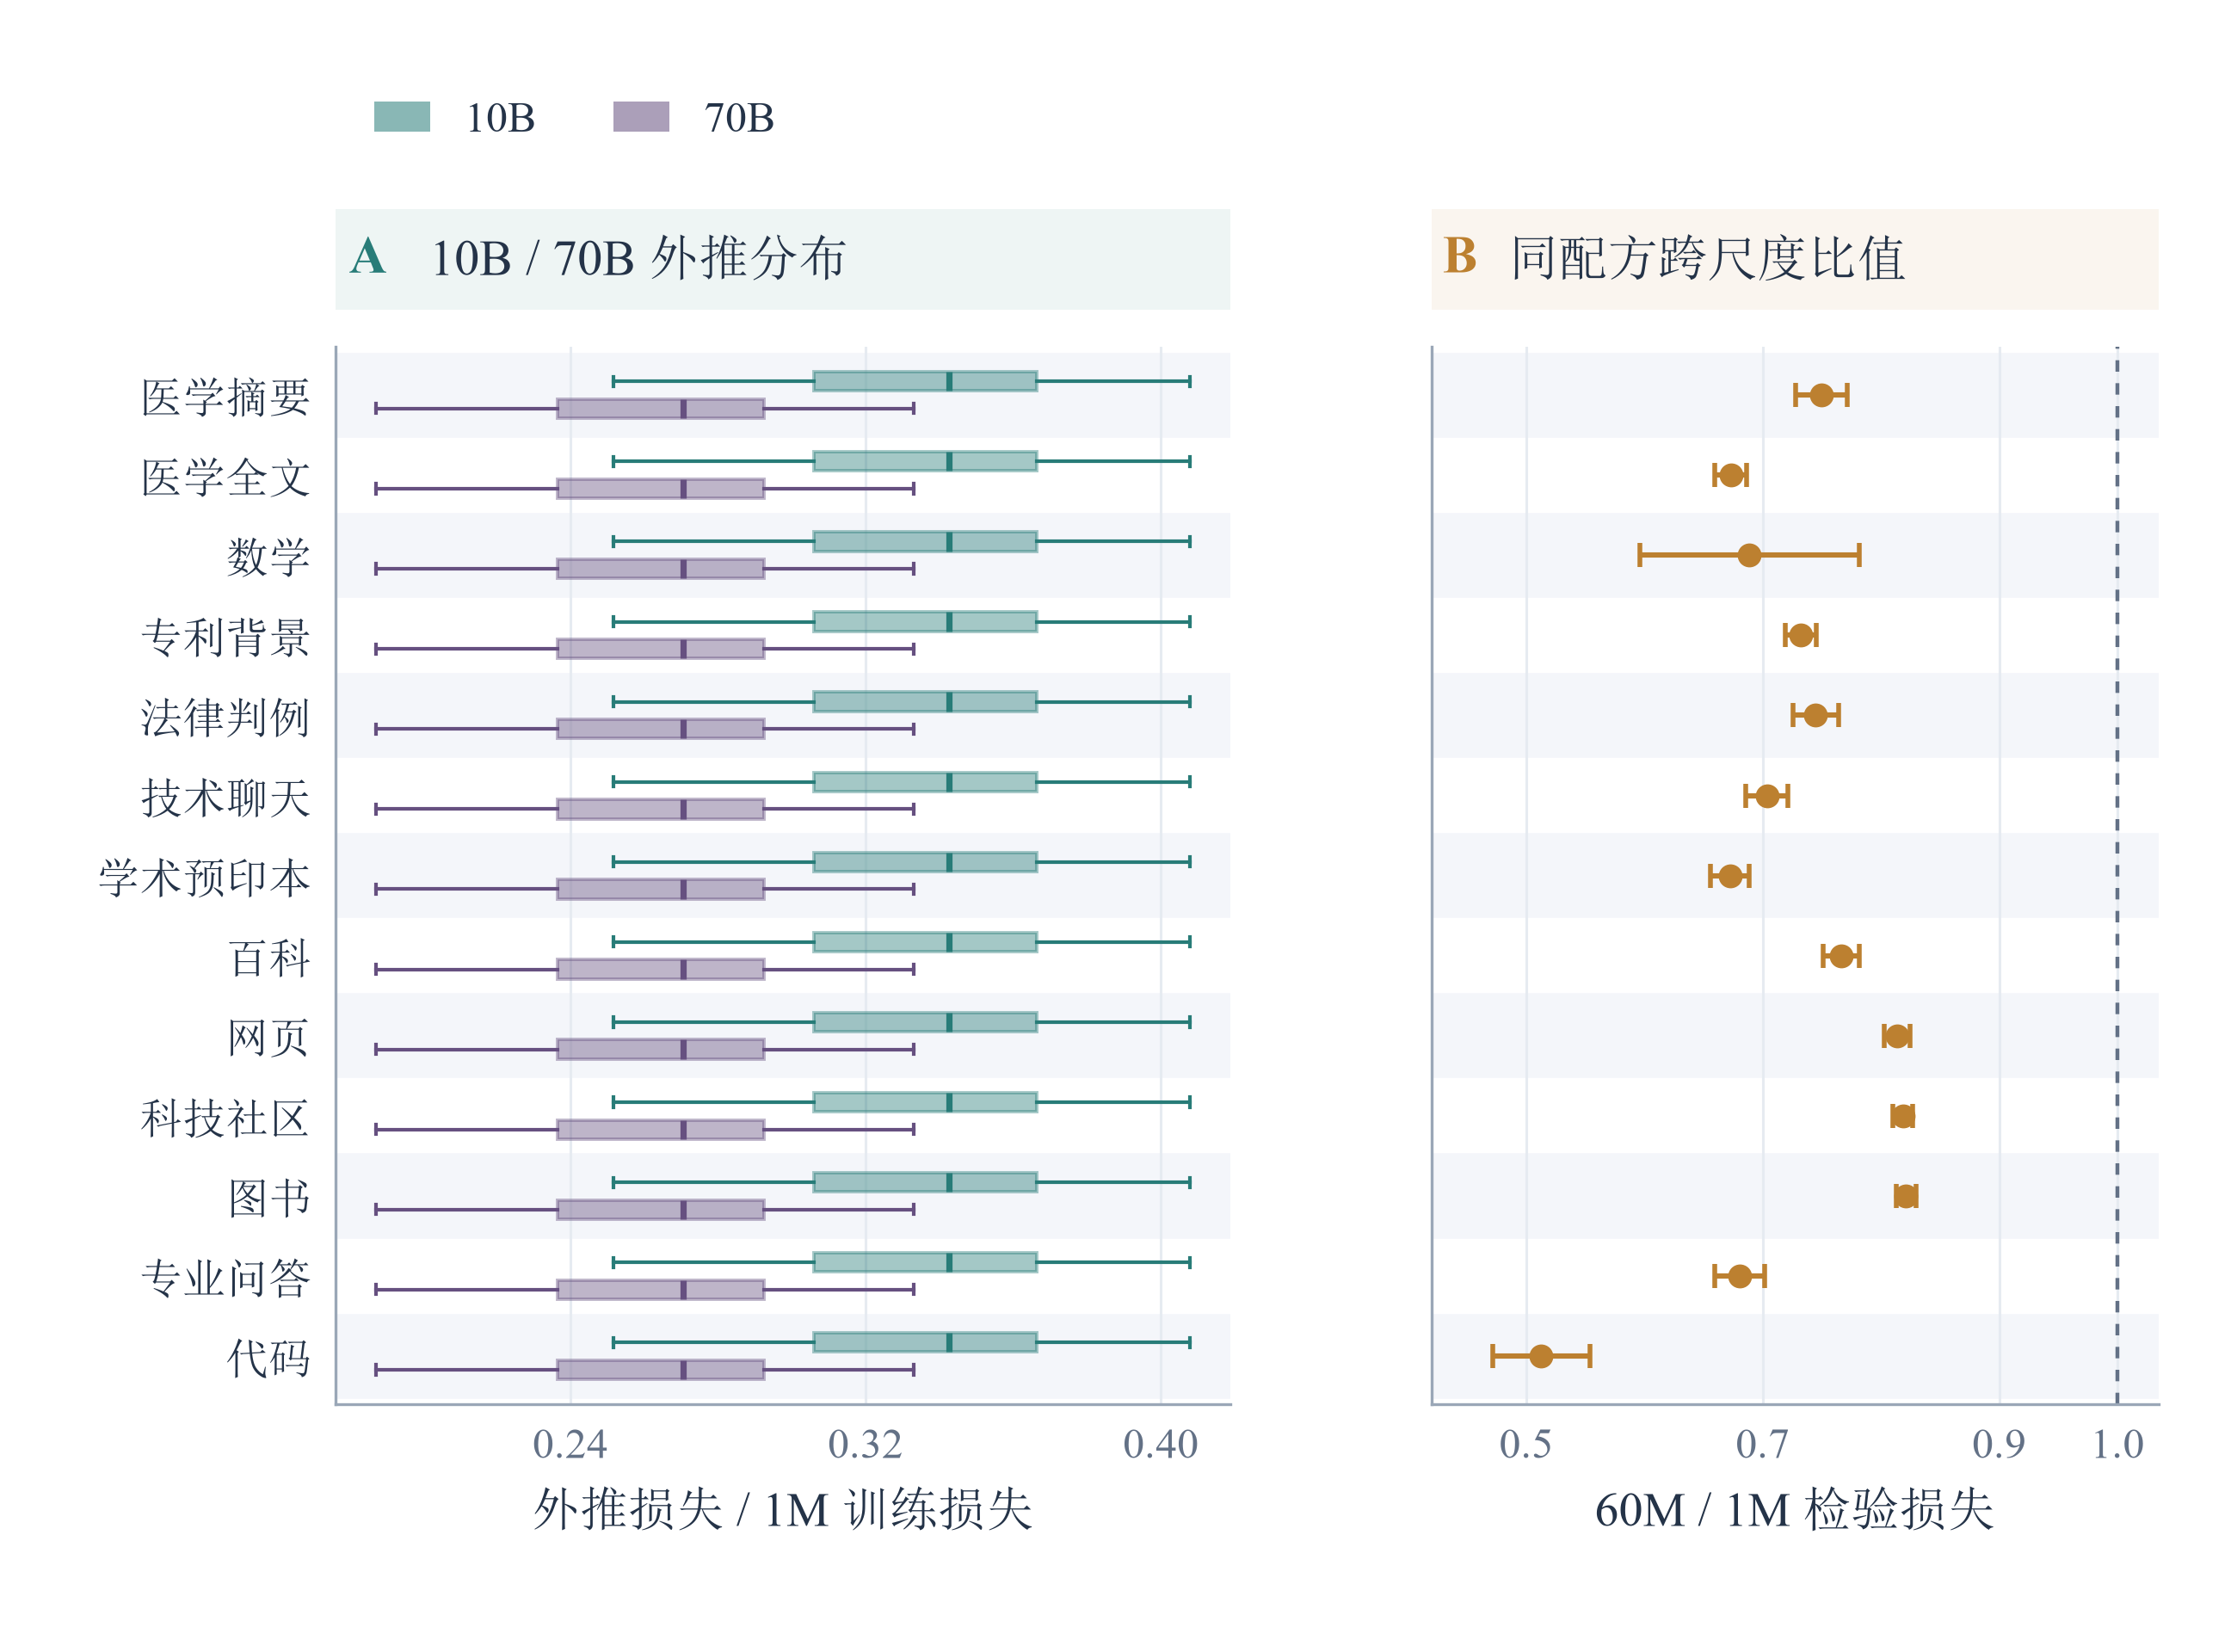
\includegraphics[width=0.92\textwidth]{../求解/问题一/图片/图7_外推与跨尺度.png}
  \caption{外推稳健性验证（左：10B 外推尺度因子；右：同配方 60M/1M 跨尺度损失比）}
  \label{fig:p1_extrap}
\end{figure}

本问得到各领域的质量分数、配比回归系数和有界推荐方案。质量对照说明评分依赖指标选择，跨规模检验说明损失还需进行尺度调整。后续资源配置将使用这些结果，并保留相应的适用条件。

\FloatBarrier
\endgroup
